% lecture5.tex -- GENERATED by build_L5.py from L5_numbers.json; do not edit by hand.
\documentclass[10pt,aspectratio=169,t]{beamer}
% =============================================================================
% emqa_preamble.tex -- shared Beamer preamble of Energy Markets Quantitative Analysis (EMQA)
% Used by every lecture: lectures/Lk/lecturek.tex does
%   \documentclass[10pt,aspectratio=169,t]{beamer}
%   % =============================================================================
% emqa_preamble.tex -- shared Beamer preamble of Energy Markets Quantitative Analysis (EMQA)
% Used by every lecture: lectures/Lk/lecturek.tex does
%   \documentclass[10pt,aspectratio=169,t]{beamer}
%   % =============================================================================
% emqa_preamble.tex -- shared Beamer preamble of Energy Markets Quantitative Analysis (EMQA)
% Used by every lecture: lectures/Lk/lecturek.tex does
%   \documentclass[10pt,aspectratio=169,t]{beamer}
%   \input{../common/emqa_preamble}
%   \emqalecture{k}{Lecture title}
% Logos live in lectures/common/logos/, charts in lectures/Lk/charts/.
% Do NOT add \hfuzz / \vfuzz / \hbadness here: overfull boxes must be fixed, not hidden.
% =============================================================================

\usetheme{default}
\setbeamersize{text margin left=7mm, text margin right=7mm}

% ---------------------------------------------------------------- packages
\usepackage[utf8]{inputenc}
\usepackage[T1]{fontenc}
\usepackage{lmodern}
\usepackage{amsmath, amssymb}
\usepackage{mathtools}
\usepackage{bm}
\usepackage{tikz}
\usetikzlibrary{arrows.meta, positioning, calc, shapes.misc}
\usepackage{booktabs}
\usepackage{array}
\usepackage{graphicx}
\usepackage{colortbl}
\usepackage{xcolor}
\usepackage{multicol}
\hypersetup{colorlinks=true, linkcolor=MainBlue, urlcolor=MainBlue, citecolor=MainBlue}
\graphicspath{{../common/logos/}}   % charts are included with their language folder: charts/en/, charts/ro/

% ---------------------------------------------------------------- colours
\definecolor{MainBlue}{RGB}{26, 58, 110}
\definecolor{IDAred}{RGB}{205, 0, 0}
\definecolor{DarkGray}{RGB}{51, 51, 51}
\definecolor{FooterGray}{RGB}{100, 100, 100}
\definecolor{BlockGray}{RGB}{236, 238, 242}
\definecolor{KeynoteGray}{RGB}{218, 218, 218}
\definecolor{Crimson}{RGB}{190, 40, 50}
\definecolor{Forest}{RGB}{30, 110, 50}
\definecolor{Bitter}{RGB}{214, 150, 20}
% chart palette (same hex values as lectures/common/emqa_plot.py)
\definecolor{SerRO}{HTML}{2A78D6}
\definecolor{SerDE}{HTML}{EB6834}
\definecolor{SerHU}{HTML}{1BAF7A}
\definecolor{SerBG}{HTML}{EDA100}

\setbeamertemplate{background}{%
  \begin{tikzpicture}[remember picture, overlay]
    \shade[shading=axis, shading angle=315, top color=white, bottom color=KeynoteGray]
      (current page.south west) rectangle (current page.north east);
  \end{tikzpicture}}
\setbeamercolor{background canvas}{bg=}
\setbeamercolor{structure}{fg=MainBlue}
\setbeamercolor{normal text}{fg=DarkGray}
\setbeamercolor{title}{fg=IDAred}
\setbeamercolor{frametitle}{fg=IDAred, bg=}
\setbeamercolor{block title}{bg=MainBlue, fg=white}
\setbeamercolor{block body}{bg=BlockGray, fg=DarkGray}
\setbeamercolor{block title alerted}{bg=Crimson, fg=white}
\setbeamercolor{block body alerted}{bg=Crimson!7, fg=DarkGray}
\setbeamercolor{block title example}{bg=Forest, fg=white}
\setbeamercolor{block body example}{bg=Forest!7, fg=DarkGray}
\setbeamercolor{item}{fg=MainBlue}
\setbeamerfont{frametitle}{size=\large, series=\bfseries}
\setbeamerfont{block title}{size=\small, series=\bfseries}
\setbeamertemplate{blocks}[rounded][shadow=false]
\setbeamertemplate{itemize item}{\color{MainBlue}$\boxdot$}
\setbeamertemplate{itemize subitem}{\color{MainBlue}\scriptsize$\blacktriangleright$}
% compact two-level lists: level 1 = main point, level 2 = details (no text outside bullets)
\setbeamerfont{itemize/enumerate subbody}{size=\footnotesize}
\setlength{\leftmargini}{1.1em}
\setlength{\leftmarginii}{1.1em}
\setbeamertemplate{itemize/enumerate body begin}{\setlength{\topsep}{0pt}\setlength{\partopsep}{0pt}\setlength{\parskip}{0pt}}
\setbeamertemplate{itemize/enumerate subbody begin}{\setlength{\topsep}{0pt}\setlength{\partopsep}{0pt}\setlength{\itemsep}{0pt}\vspace{-0.4ex}}

\setbeamertemplate{enumerate item}{\color{MainBlue}\insertenumlabel.}
\setlength{\leftmargini}{1.3em}
\setlength{\leftmarginii}{1.2em}
\setbeamertemplate{navigation symbols}{}
\setbeamertemplate{section in toc}{\color{MainBlue}$\blacktriangleright$~\inserttocsection}
\setbeamertemplate{caption}{\raggedright\insertcaption\par}
% frame subtitle = precise citation line under the claim title (Weron style)
\setbeamerfont{framesubtitle}{size=\footnotesize}
\setbeamercolor{framesubtitle}{fg=FooterGray}
% outline that reappears at every section with the current section highlighted
\setbeamertemplate{section in toc shaded}[default][35]
\setbeamertemplate{subsection in toc shaded}[default][35]
\setbeamertemplate{subsection in toc}{\leavevmode\leftskip=2.2em\color{DarkGray}\small\inserttocsubsection\par}
\AtBeginSection[]{{\begin{frame}{\txtoutline}\vspace{2mm}\small
  \tableofcontents[currentsection,hideothersubsections]\end{frame}}}

% ---------------------------------------------------------------- head and foot
\setbeamertemplate{headline}{%
  \vskip10pt%
  \hbox to \paperwidth{\hskip0.5cm%
    {\small\color{FooterGray}\renewcommand{\hyperlink}[2]{##2}\insertsectionhead}%
    \hfill\textcolor{FooterGray}{\small\insertframenumber}\hskip0.5cm}%
  \vskip4pt{\color{FooterGray}\hrule height 0.4pt}}
% footer as in the other courses (MFM, SFM): course name on the left, small sparkline on the right
\setbeamertemplate{footline}{%
  {\color{FooterGray}\hrule height 0.4pt}\vskip4pt%
  \hbox to \paperwidth{\hskip0.5cm%
    \textcolor{FooterGray}{\small\txtcourse}%
    \hfill\raisebox{-0.1em}{\begin{tikzpicture}[x=0.08em, y=0.08em, line width=0.4pt]
      \draw[FooterGray] (0,3) -- (1,4) -- (2,3.5) -- (3,5) -- (4,4) -- (5,6) -- (6,5.5) -- (7,4) -- (8,5) -- (9,7) -- (10,6) -- (11,5) -- (12,6.5) -- (13,8) -- (14,7) -- (15,6) -- (16,7.5) -- (17,9) -- (18,8) -- (19,7) -- (20,8.5) -- (21,10) -- (22,9) -- (23,8) -- (24,9.5);
    \end{tikzpicture}}\hskip0.5cm}%
  \vskip6pt}

% ---------------------------------------------------------------- title page
\defbeamertemplate*{title page}{emqa}[1][]{%
  \vspace{0.15cm}
  \begin{center}
    \href{https://www.ase.ro}{
\includegraphics[height=0.9cm]{ase_logo.png}}\hspace{0.3cm}%
    \href{https://ipe.ro/new}{
\includegraphics[height=0.9cm]{acad_logo.png}}\hspace{0.3cm}%
    \href{https://theida.net}{
\includegraphics[height=0.9cm]{ida_logo.png}}\hspace{0.3cm}%
    \href{https://blockchain-research-center.com}{
\includegraphics[height=0.9cm]{brc_logo.png}}\hspace{0.3cm}%
    \href{https://www.ai4efin.ase.ro}{
\includegraphics[height=0.9cm]{ai4efin_logo.png}}\hspace{0.3cm}%
    \href{https://www.digital-finance-msca.com}{
\includegraphics[height=0.9cm]{msca_logo.png}}%
  \end{center}
  \vspace{0.45cm}
  \begin{center}
    \begin{minipage}{0.1\textwidth}\centering
      \href{https://quantlet.com}{
\includegraphics[height=0.9cm]{ql_logo.png}}\end{minipage}%
    \begin{minipage}{0.78\textwidth}\centering
      {\Large\bfseries\usebeamercolor[fg]{title}\inserttitle}\par\vspace{0.25cm}
      {\large\usebeamercolor[fg]{title}\insertsubtitle}\end{minipage}%
    \begin{minipage}{0.1\textwidth}\centering
      \href{https://quantinar.com}{
\includegraphics[height=0.9cm]{qr_logo.png}}\end{minipage}
  \end{center}
  \vfill
  \hspace{0.4cm}{\bfseries\insertauthor}\par\vspace{0.12cm}
  \hspace{0.4cm}\begin{minipage}[t]{0.92\textwidth}\raggedright\footnotesize\insertinstitute\end{minipage}
  \par\vspace{0.4cm}}

% ---------------------------------------------------------------- lecture metadata
\newcommand{\emqashort}{}
\newcommand{\emqanb}{notebooks}
\newcommand{\emqarepo}{https://github.com/danpele/EMQA/tree/main}
% language-dependent labels (English default; \emqaromanian switches to Romanian, call it before \emqalecture)
\newcommand{\txtcourse}{Energy Markets Quantitative Analysis}
\newcommand{\txtlecture}{Lecture}
\newcommand{\txtoutline}{Outline}
\newcommand{\txtintuition}{In one sentence:}
\newcommand{\txtjob}{In practice:}
\newcommand{\txttry}{Experiment yourself:}
\newcommand{\txtwhere}{where}
\newcommand{\txtsim}{SIMULATED DATA (teaching illustration)}
\newcommand{\txtnbsuffix}{}
\newcommand{\txtinstitute}{Bucharest University of Economic Studies, Department of Statistics and Econometrics\\
    Romanian Academy, Institute for Economic Forecasting\\
    IDA Institute Digital Assets \textbullet\ AI4EFin \textbullet\ MSCA Digital Finance}
\newcommand{\emqaromanian}{%
  \renewcommand{\txtcourse}{Analiza cantitativă a piețelor de energie}%
  \renewcommand{\txtlecture}{Cursul}%
  \renewcommand{\txtoutline}{Cuprins}%
  \renewcommand{\txtintuition}{Pe scurt:}%
  \renewcommand{\txtjob}{În practică:}%
  \renewcommand{\txttry}{Exercițiu practic:}%
  \renewcommand{\txtwhere}{unde}%
  \renewcommand{\txtsim}{DATE SIMULATE (doar pentru ilustrare)}%
  \renewcommand{\txtnbsuffix}{\string_ro}%
  \renewcommand{\txtinstitute}{Academia de Studii Economice din București, Departamentul de Statistică și Econometrie\\
    Academia Română, Institutul de Prognoză Economică\\
    IDA Institute Digital Assets \textbullet\ AI4EFin \textbullet\ MSCA Digital Finance}}
\newcommand{\emqalecture}[2]{%
  \renewcommand{\emqashort}{\txtlecture\ #1}%
  \renewcommand{\emqanb}{notebooks/L#1\string_notebook\txtnbsuffix.ipynb}%
  \title[EMQA]{\txtcourse}%
  \subtitle{\txtlecture\ #1: #2}%
  \author{Prof.\ dr.\ Daniel Traian PELE}%
  \institute{\txtinstitute}%
  \date{}}

% ---------------------------------------------------------------- teaching blocks (MBA clarity rule)
% \intuition{one plain sentence}  ->  formula with every symbol defined  ->  real-data example  ->  \manager{one line}
\newcommand{\intuition}[1]{\begin{itemize}\item {\color{MainBlue}\textbf{\txtintuition}}~#1\end{itemize}\vspace{0.6mm}}
\newcommand{\manager}[1]{\colorbox{Forest!10}{\parbox{\dimexpr\linewidth-2\fboxsep\relax}{\footnotesize
  \begin{itemize}\setlength{\itemsep}{0pt}\item \textbf{\color{Forest}\txtjob}~#1\end{itemize}}}}
% Experiment yourself: pointer to the matching notebook section
\newcommand{\tryit}[1]{{\scriptsize\href{\emqarepo/\emqanb}{%
  \raisebox{-0.15em}{
\includegraphics[height=0.85em]{ql_logo.png}}\,\textbf{\txttry}~\color{MainBlue}#1}}}
% bottom row: manager line (left) + experiment pointer (right), pinned to the bottom of the frame
\newcommand{\bottomrow}[2]{\par\vfill\noindent\begin{minipage}[b]{0.72\linewidth}#1\end{minipage}\hfill
  \begin{minipage}[b]{0.26\linewidth}\raggedleft #2\end{minipage}\par\vspace{0.5mm}}
\newcommand{\where}[1]{{\footnotesize\textbf{\txtwhere}~#1\par}}

% ---------------------------------------------------------------- helpers
% chart source line under a figure: \chartsource{Source ...; period ...}
\newcommand{\chartsource}[1]{\par\vspace{1pt}{\scriptsize\color{FooterGray}#1\par}}
% link to code: \quantlet{label}{path inside the repo}
\newcommand{\quantlet}[2]{\par\vspace{1pt}\hfill\href{\emqarepo/#2}{%
  \raisebox{-0.15em}{
\includegraphics[height=0.75em]{ql_logo.png}}\textcolor{MainBlue}{\scriptsize\ #1}}}
\newcommand{\simlabel}{\colorbox{Crimson!12}{\scriptsize\bfseries\color{Crimson}\txtsim}}
\newcommand{\E}{\mathbb{E}}
\newcommand{\Var}{\operatorname{Var}}
\newcommand{\Cov}{\operatorname{Cov}}
\newcommand{\Corr}{\operatorname{Corr}}
\newcommand{\asinh}{\operatorname{asinh}}
\newcommand{\iid}{\overset{\text{i.i.d.}}{\sim}}
\newcommand{\EUR}{EUR}

%   \emqalecture{k}{Lecture title}
% Logos live in lectures/common/logos/, charts in lectures/Lk/charts/.
% Do NOT add \hfuzz / \vfuzz / \hbadness here: overfull boxes must be fixed, not hidden.
% =============================================================================

\usetheme{default}
\setbeamersize{text margin left=7mm, text margin right=7mm}

% ---------------------------------------------------------------- packages
\usepackage[utf8]{inputenc}
\usepackage[T1]{fontenc}
\usepackage{lmodern}
\usepackage{amsmath, amssymb}
\usepackage{mathtools}
\usepackage{bm}
\usepackage{tikz}
\usetikzlibrary{arrows.meta, positioning, calc, shapes.misc}
\usepackage{booktabs}
\usepackage{array}
\usepackage{graphicx}
\usepackage{colortbl}
\usepackage{xcolor}
\usepackage{multicol}
\hypersetup{colorlinks=true, linkcolor=MainBlue, urlcolor=MainBlue, citecolor=MainBlue}
\graphicspath{{../common/logos/}}   % charts are included with their language folder: charts/en/, charts/ro/

% ---------------------------------------------------------------- colours
\definecolor{MainBlue}{RGB}{26, 58, 110}
\definecolor{IDAred}{RGB}{205, 0, 0}
\definecolor{DarkGray}{RGB}{51, 51, 51}
\definecolor{FooterGray}{RGB}{100, 100, 100}
\definecolor{BlockGray}{RGB}{236, 238, 242}
\definecolor{KeynoteGray}{RGB}{218, 218, 218}
\definecolor{Crimson}{RGB}{190, 40, 50}
\definecolor{Forest}{RGB}{30, 110, 50}
\definecolor{Bitter}{RGB}{214, 150, 20}
% chart palette (same hex values as lectures/common/emqa_plot.py)
\definecolor{SerRO}{HTML}{2A78D6}
\definecolor{SerDE}{HTML}{EB6834}
\definecolor{SerHU}{HTML}{1BAF7A}
\definecolor{SerBG}{HTML}{EDA100}

\setbeamertemplate{background}{%
  \begin{tikzpicture}[remember picture, overlay]
    \shade[shading=axis, shading angle=315, top color=white, bottom color=KeynoteGray]
      (current page.south west) rectangle (current page.north east);
  \end{tikzpicture}}
\setbeamercolor{background canvas}{bg=}
\setbeamercolor{structure}{fg=MainBlue}
\setbeamercolor{normal text}{fg=DarkGray}
\setbeamercolor{title}{fg=IDAred}
\setbeamercolor{frametitle}{fg=IDAred, bg=}
\setbeamercolor{block title}{bg=MainBlue, fg=white}
\setbeamercolor{block body}{bg=BlockGray, fg=DarkGray}
\setbeamercolor{block title alerted}{bg=Crimson, fg=white}
\setbeamercolor{block body alerted}{bg=Crimson!7, fg=DarkGray}
\setbeamercolor{block title example}{bg=Forest, fg=white}
\setbeamercolor{block body example}{bg=Forest!7, fg=DarkGray}
\setbeamercolor{item}{fg=MainBlue}
\setbeamerfont{frametitle}{size=\large, series=\bfseries}
\setbeamerfont{block title}{size=\small, series=\bfseries}
\setbeamertemplate{blocks}[rounded][shadow=false]
\setbeamertemplate{itemize item}{\color{MainBlue}$\boxdot$}
\setbeamertemplate{itemize subitem}{\color{MainBlue}\scriptsize$\blacktriangleright$}
% compact two-level lists: level 1 = main point, level 2 = details (no text outside bullets)
\setbeamerfont{itemize/enumerate subbody}{size=\footnotesize}
\setlength{\leftmargini}{1.1em}
\setlength{\leftmarginii}{1.1em}
\setbeamertemplate{itemize/enumerate body begin}{\setlength{\topsep}{0pt}\setlength{\partopsep}{0pt}\setlength{\parskip}{0pt}}
\setbeamertemplate{itemize/enumerate subbody begin}{\setlength{\topsep}{0pt}\setlength{\partopsep}{0pt}\setlength{\itemsep}{0pt}\vspace{-0.4ex}}

\setbeamertemplate{enumerate item}{\color{MainBlue}\insertenumlabel.}
\setlength{\leftmargini}{1.3em}
\setlength{\leftmarginii}{1.2em}
\setbeamertemplate{navigation symbols}{}
\setbeamertemplate{section in toc}{\color{MainBlue}$\blacktriangleright$~\inserttocsection}
\setbeamertemplate{caption}{\raggedright\insertcaption\par}
% frame subtitle = precise citation line under the claim title (Weron style)
\setbeamerfont{framesubtitle}{size=\footnotesize}
\setbeamercolor{framesubtitle}{fg=FooterGray}
% outline that reappears at every section with the current section highlighted
\setbeamertemplate{section in toc shaded}[default][35]
\setbeamertemplate{subsection in toc shaded}[default][35]
\setbeamertemplate{subsection in toc}{\leavevmode\leftskip=2.2em\color{DarkGray}\small\inserttocsubsection\par}
\AtBeginSection[]{{\begin{frame}{\txtoutline}\vspace{2mm}\small
  \tableofcontents[currentsection,hideothersubsections]\end{frame}}}

% ---------------------------------------------------------------- head and foot
\setbeamertemplate{headline}{%
  \vskip10pt%
  \hbox to \paperwidth{\hskip0.5cm%
    {\small\color{FooterGray}\renewcommand{\hyperlink}[2]{##2}\insertsectionhead}%
    \hfill\textcolor{FooterGray}{\small\insertframenumber}\hskip0.5cm}%
  \vskip4pt{\color{FooterGray}\hrule height 0.4pt}}
% footer as in the other courses (MFM, SFM): course name on the left, small sparkline on the right
\setbeamertemplate{footline}{%
  {\color{FooterGray}\hrule height 0.4pt}\vskip4pt%
  \hbox to \paperwidth{\hskip0.5cm%
    \textcolor{FooterGray}{\small\txtcourse}%
    \hfill\raisebox{-0.1em}{\begin{tikzpicture}[x=0.08em, y=0.08em, line width=0.4pt]
      \draw[FooterGray] (0,3) -- (1,4) -- (2,3.5) -- (3,5) -- (4,4) -- (5,6) -- (6,5.5) -- (7,4) -- (8,5) -- (9,7) -- (10,6) -- (11,5) -- (12,6.5) -- (13,8) -- (14,7) -- (15,6) -- (16,7.5) -- (17,9) -- (18,8) -- (19,7) -- (20,8.5) -- (21,10) -- (22,9) -- (23,8) -- (24,9.5);
    \end{tikzpicture}}\hskip0.5cm}%
  \vskip6pt}

% ---------------------------------------------------------------- title page
\defbeamertemplate*{title page}{emqa}[1][]{%
  \vspace{0.15cm}
  \begin{center}
    \href{https://www.ase.ro}{
\includegraphics[height=0.9cm]{ase_logo.png}}\hspace{0.3cm}%
    \href{https://ipe.ro/new}{
\includegraphics[height=0.9cm]{acad_logo.png}}\hspace{0.3cm}%
    \href{https://theida.net}{
\includegraphics[height=0.9cm]{ida_logo.png}}\hspace{0.3cm}%
    \href{https://blockchain-research-center.com}{
\includegraphics[height=0.9cm]{brc_logo.png}}\hspace{0.3cm}%
    \href{https://www.ai4efin.ase.ro}{
\includegraphics[height=0.9cm]{ai4efin_logo.png}}\hspace{0.3cm}%
    \href{https://www.digital-finance-msca.com}{
\includegraphics[height=0.9cm]{msca_logo.png}}%
  \end{center}
  \vspace{0.45cm}
  \begin{center}
    \begin{minipage}{0.1\textwidth}\centering
      \href{https://quantlet.com}{
\includegraphics[height=0.9cm]{ql_logo.png}}\end{minipage}%
    \begin{minipage}{0.78\textwidth}\centering
      {\Large\bfseries\usebeamercolor[fg]{title}\inserttitle}\par\vspace{0.25cm}
      {\large\usebeamercolor[fg]{title}\insertsubtitle}\end{minipage}%
    \begin{minipage}{0.1\textwidth}\centering
      \href{https://quantinar.com}{
\includegraphics[height=0.9cm]{qr_logo.png}}\end{minipage}
  \end{center}
  \vfill
  \hspace{0.4cm}{\bfseries\insertauthor}\par\vspace{0.12cm}
  \hspace{0.4cm}\begin{minipage}[t]{0.92\textwidth}\raggedright\footnotesize\insertinstitute\end{minipage}
  \par\vspace{0.4cm}}

% ---------------------------------------------------------------- lecture metadata
\newcommand{\emqashort}{}
\newcommand{\emqanb}{notebooks}
\newcommand{\emqarepo}{https://github.com/danpele/EMQA/tree/main}
% language-dependent labels (English default; \emqaromanian switches to Romanian, call it before \emqalecture)
\newcommand{\txtcourse}{Energy Markets Quantitative Analysis}
\newcommand{\txtlecture}{Lecture}
\newcommand{\txtoutline}{Outline}
\newcommand{\txtintuition}{In one sentence:}
\newcommand{\txtjob}{In practice:}
\newcommand{\txttry}{Experiment yourself:}
\newcommand{\txtwhere}{where}
\newcommand{\txtsim}{SIMULATED DATA (teaching illustration)}
\newcommand{\txtnbsuffix}{}
\newcommand{\txtinstitute}{Bucharest University of Economic Studies, Department of Statistics and Econometrics\\
    Romanian Academy, Institute for Economic Forecasting\\
    IDA Institute Digital Assets \textbullet\ AI4EFin \textbullet\ MSCA Digital Finance}
\newcommand{\emqaromanian}{%
  \renewcommand{\txtcourse}{Analiza cantitativă a piețelor de energie}%
  \renewcommand{\txtlecture}{Cursul}%
  \renewcommand{\txtoutline}{Cuprins}%
  \renewcommand{\txtintuition}{Pe scurt:}%
  \renewcommand{\txtjob}{În practică:}%
  \renewcommand{\txttry}{Exercițiu practic:}%
  \renewcommand{\txtwhere}{unde}%
  \renewcommand{\txtsim}{DATE SIMULATE (doar pentru ilustrare)}%
  \renewcommand{\txtnbsuffix}{\string_ro}%
  \renewcommand{\txtinstitute}{Academia de Studii Economice din București, Departamentul de Statistică și Econometrie\\
    Academia Română, Institutul de Prognoză Economică\\
    IDA Institute Digital Assets \textbullet\ AI4EFin \textbullet\ MSCA Digital Finance}}
\newcommand{\emqalecture}[2]{%
  \renewcommand{\emqashort}{\txtlecture\ #1}%
  \renewcommand{\emqanb}{notebooks/L#1\string_notebook\txtnbsuffix.ipynb}%
  \title[EMQA]{\txtcourse}%
  \subtitle{\txtlecture\ #1: #2}%
  \author{Prof.\ dr.\ Daniel Traian PELE}%
  \institute{\txtinstitute}%
  \date{}}

% ---------------------------------------------------------------- teaching blocks (MBA clarity rule)
% \intuition{one plain sentence}  ->  formula with every symbol defined  ->  real-data example  ->  \manager{one line}
\newcommand{\intuition}[1]{\begin{itemize}\item {\color{MainBlue}\textbf{\txtintuition}}~#1\end{itemize}\vspace{0.6mm}}
\newcommand{\manager}[1]{\colorbox{Forest!10}{\parbox{\dimexpr\linewidth-2\fboxsep\relax}{\footnotesize
  \begin{itemize}\setlength{\itemsep}{0pt}\item \textbf{\color{Forest}\txtjob}~#1\end{itemize}}}}
% Experiment yourself: pointer to the matching notebook section
\newcommand{\tryit}[1]{{\scriptsize\href{\emqarepo/\emqanb}{%
  \raisebox{-0.15em}{
\includegraphics[height=0.85em]{ql_logo.png}}\,\textbf{\txttry}~\color{MainBlue}#1}}}
% bottom row: manager line (left) + experiment pointer (right), pinned to the bottom of the frame
\newcommand{\bottomrow}[2]{\par\vfill\noindent\begin{minipage}[b]{0.72\linewidth}#1\end{minipage}\hfill
  \begin{minipage}[b]{0.26\linewidth}\raggedleft #2\end{minipage}\par\vspace{0.5mm}}
\newcommand{\where}[1]{{\footnotesize\textbf{\txtwhere}~#1\par}}

% ---------------------------------------------------------------- helpers
% chart source line under a figure: \chartsource{Source ...; period ...}
\newcommand{\chartsource}[1]{\par\vspace{1pt}{\scriptsize\color{FooterGray}#1\par}}
% link to code: \quantlet{label}{path inside the repo}
\newcommand{\quantlet}[2]{\par\vspace{1pt}\hfill\href{\emqarepo/#2}{%
  \raisebox{-0.15em}{
\includegraphics[height=0.75em]{ql_logo.png}}\textcolor{MainBlue}{\scriptsize\ #1}}}
\newcommand{\simlabel}{\colorbox{Crimson!12}{\scriptsize\bfseries\color{Crimson}\txtsim}}
\newcommand{\E}{\mathbb{E}}
\newcommand{\Var}{\operatorname{Var}}
\newcommand{\Cov}{\operatorname{Cov}}
\newcommand{\Corr}{\operatorname{Corr}}
\newcommand{\asinh}{\operatorname{asinh}}
\newcommand{\iid}{\overset{\text{i.i.d.}}{\sim}}
\newcommand{\EUR}{EUR}

%   \emqalecture{k}{Lecture title}
% Logos live in lectures/common/logos/, charts in lectures/Lk/charts/.
% Do NOT add \hfuzz / \vfuzz / \hbadness here: overfull boxes must be fixed, not hidden.
% =============================================================================

\usetheme{default}
\setbeamersize{text margin left=7mm, text margin right=7mm}

% ---------------------------------------------------------------- packages
\usepackage[utf8]{inputenc}
\usepackage[T1]{fontenc}
\usepackage{lmodern}
\usepackage{amsmath, amssymb}
\usepackage{mathtools}
\usepackage{bm}
\usepackage{tikz}
\usetikzlibrary{arrows.meta, positioning, calc, shapes.misc}
\usepackage{booktabs}
\usepackage{array}
\usepackage{graphicx}
\usepackage{colortbl}
\usepackage{xcolor}
\usepackage{multicol}
\hypersetup{colorlinks=true, linkcolor=MainBlue, urlcolor=MainBlue, citecolor=MainBlue}
\graphicspath{{../common/logos/}}   % charts are included with their language folder: charts/en/, charts/ro/

% ---------------------------------------------------------------- colours
\definecolor{MainBlue}{RGB}{26, 58, 110}
\definecolor{IDAred}{RGB}{205, 0, 0}
\definecolor{DarkGray}{RGB}{51, 51, 51}
\definecolor{FooterGray}{RGB}{100, 100, 100}
\definecolor{BlockGray}{RGB}{236, 238, 242}
\definecolor{KeynoteGray}{RGB}{218, 218, 218}
\definecolor{Crimson}{RGB}{190, 40, 50}
\definecolor{Forest}{RGB}{30, 110, 50}
\definecolor{Bitter}{RGB}{214, 150, 20}
% chart palette (same hex values as lectures/common/emqa_plot.py)
\definecolor{SerRO}{HTML}{2A78D6}
\definecolor{SerDE}{HTML}{EB6834}
\definecolor{SerHU}{HTML}{1BAF7A}
\definecolor{SerBG}{HTML}{EDA100}

\setbeamertemplate{background}{%
  \begin{tikzpicture}[remember picture, overlay]
    \shade[shading=axis, shading angle=315, top color=white, bottom color=KeynoteGray]
      (current page.south west) rectangle (current page.north east);
  \end{tikzpicture}}
\setbeamercolor{background canvas}{bg=}
\setbeamercolor{structure}{fg=MainBlue}
\setbeamercolor{normal text}{fg=DarkGray}
\setbeamercolor{title}{fg=IDAred}
\setbeamercolor{frametitle}{fg=IDAred, bg=}
\setbeamercolor{block title}{bg=MainBlue, fg=white}
\setbeamercolor{block body}{bg=BlockGray, fg=DarkGray}
\setbeamercolor{block title alerted}{bg=Crimson, fg=white}
\setbeamercolor{block body alerted}{bg=Crimson!7, fg=DarkGray}
\setbeamercolor{block title example}{bg=Forest, fg=white}
\setbeamercolor{block body example}{bg=Forest!7, fg=DarkGray}
\setbeamercolor{item}{fg=MainBlue}
\setbeamerfont{frametitle}{size=\large, series=\bfseries}
\setbeamerfont{block title}{size=\small, series=\bfseries}
\setbeamertemplate{blocks}[rounded][shadow=false]
\setbeamertemplate{itemize item}{\color{MainBlue}$\boxdot$}
\setbeamertemplate{itemize subitem}{\color{MainBlue}\scriptsize$\blacktriangleright$}
% compact two-level lists: level 1 = main point, level 2 = details (no text outside bullets)
\setbeamerfont{itemize/enumerate subbody}{size=\footnotesize}
\setlength{\leftmargini}{1.1em}
\setlength{\leftmarginii}{1.1em}
\setbeamertemplate{itemize/enumerate body begin}{\setlength{\topsep}{0pt}\setlength{\partopsep}{0pt}\setlength{\parskip}{0pt}}
\setbeamertemplate{itemize/enumerate subbody begin}{\setlength{\topsep}{0pt}\setlength{\partopsep}{0pt}\setlength{\itemsep}{0pt}\vspace{-0.4ex}}

\setbeamertemplate{enumerate item}{\color{MainBlue}\insertenumlabel.}
\setlength{\leftmargini}{1.3em}
\setlength{\leftmarginii}{1.2em}
\setbeamertemplate{navigation symbols}{}
\setbeamertemplate{section in toc}{\color{MainBlue}$\blacktriangleright$~\inserttocsection}
\setbeamertemplate{caption}{\raggedright\insertcaption\par}
% frame subtitle = precise citation line under the claim title (Weron style)
\setbeamerfont{framesubtitle}{size=\footnotesize}
\setbeamercolor{framesubtitle}{fg=FooterGray}
% outline that reappears at every section with the current section highlighted
\setbeamertemplate{section in toc shaded}[default][35]
\setbeamertemplate{subsection in toc shaded}[default][35]
\setbeamertemplate{subsection in toc}{\leavevmode\leftskip=2.2em\color{DarkGray}\small\inserttocsubsection\par}
\AtBeginSection[]{{\begin{frame}{\txtoutline}\vspace{2mm}\small
  \tableofcontents[currentsection,hideothersubsections]\end{frame}}}

% ---------------------------------------------------------------- head and foot
\setbeamertemplate{headline}{%
  \vskip10pt%
  \hbox to \paperwidth{\hskip0.5cm%
    {\small\color{FooterGray}\renewcommand{\hyperlink}[2]{##2}\insertsectionhead}%
    \hfill\textcolor{FooterGray}{\small\insertframenumber}\hskip0.5cm}%
  \vskip4pt{\color{FooterGray}\hrule height 0.4pt}}
% footer as in the other courses (MFM, SFM): course name on the left, small sparkline on the right
\setbeamertemplate{footline}{%
  {\color{FooterGray}\hrule height 0.4pt}\vskip4pt%
  \hbox to \paperwidth{\hskip0.5cm%
    \textcolor{FooterGray}{\small\txtcourse}%
    \hfill\raisebox{-0.1em}{\begin{tikzpicture}[x=0.08em, y=0.08em, line width=0.4pt]
      \draw[FooterGray] (0,3) -- (1,4) -- (2,3.5) -- (3,5) -- (4,4) -- (5,6) -- (6,5.5) -- (7,4) -- (8,5) -- (9,7) -- (10,6) -- (11,5) -- (12,6.5) -- (13,8) -- (14,7) -- (15,6) -- (16,7.5) -- (17,9) -- (18,8) -- (19,7) -- (20,8.5) -- (21,10) -- (22,9) -- (23,8) -- (24,9.5);
    \end{tikzpicture}}\hskip0.5cm}%
  \vskip6pt}

% ---------------------------------------------------------------- title page
\defbeamertemplate*{title page}{emqa}[1][]{%
  \vspace{0.15cm}
  \begin{center}
    \href{https://www.ase.ro}{
\includegraphics[height=0.9cm]{ase_logo.png}}\hspace{0.3cm}%
    \href{https://ipe.ro/new}{
\includegraphics[height=0.9cm]{acad_logo.png}}\hspace{0.3cm}%
    \href{https://theida.net}{
\includegraphics[height=0.9cm]{ida_logo.png}}\hspace{0.3cm}%
    \href{https://blockchain-research-center.com}{
\includegraphics[height=0.9cm]{brc_logo.png}}\hspace{0.3cm}%
    \href{https://www.ai4efin.ase.ro}{
\includegraphics[height=0.9cm]{ai4efin_logo.png}}\hspace{0.3cm}%
    \href{https://www.digital-finance-msca.com}{
\includegraphics[height=0.9cm]{msca_logo.png}}%
  \end{center}
  \vspace{0.45cm}
  \begin{center}
    \begin{minipage}{0.1\textwidth}\centering
      \href{https://quantlet.com}{
\includegraphics[height=0.9cm]{ql_logo.png}}\end{minipage}%
    \begin{minipage}{0.78\textwidth}\centering
      {\Large\bfseries\usebeamercolor[fg]{title}\inserttitle}\par\vspace{0.25cm}
      {\large\usebeamercolor[fg]{title}\insertsubtitle}\end{minipage}%
    \begin{minipage}{0.1\textwidth}\centering
      \href{https://quantinar.com}{
\includegraphics[height=0.9cm]{qr_logo.png}}\end{minipage}
  \end{center}
  \vfill
  \hspace{0.4cm}{\bfseries\insertauthor}\par\vspace{0.12cm}
  \hspace{0.4cm}\begin{minipage}[t]{0.92\textwidth}\raggedright\footnotesize\insertinstitute\end{minipage}
  \par\vspace{0.4cm}}

% ---------------------------------------------------------------- lecture metadata
\newcommand{\emqashort}{}
\newcommand{\emqanb}{notebooks}
\newcommand{\emqarepo}{https://github.com/danpele/EMQA/tree/main}
% language-dependent labels (English default; \emqaromanian switches to Romanian, call it before \emqalecture)
\newcommand{\txtcourse}{Energy Markets Quantitative Analysis}
\newcommand{\txtlecture}{Lecture}
\newcommand{\txtoutline}{Outline}
\newcommand{\txtintuition}{In one sentence:}
\newcommand{\txtjob}{In practice:}
\newcommand{\txttry}{Experiment yourself:}
\newcommand{\txtwhere}{where}
\newcommand{\txtsim}{SIMULATED DATA (teaching illustration)}
\newcommand{\txtnbsuffix}{}
\newcommand{\txtinstitute}{Bucharest University of Economic Studies, Department of Statistics and Econometrics\\
    Romanian Academy, Institute for Economic Forecasting\\
    IDA Institute Digital Assets \textbullet\ AI4EFin \textbullet\ MSCA Digital Finance}
\newcommand{\emqaromanian}{%
  \renewcommand{\txtcourse}{Analiza cantitativă a piețelor de energie}%
  \renewcommand{\txtlecture}{Cursul}%
  \renewcommand{\txtoutline}{Cuprins}%
  \renewcommand{\txtintuition}{Pe scurt:}%
  \renewcommand{\txtjob}{În practică:}%
  \renewcommand{\txttry}{Exercițiu practic:}%
  \renewcommand{\txtwhere}{unde}%
  \renewcommand{\txtsim}{DATE SIMULATE (doar pentru ilustrare)}%
  \renewcommand{\txtnbsuffix}{\string_ro}%
  \renewcommand{\txtinstitute}{Academia de Studii Economice din București, Departamentul de Statistică și Econometrie\\
    Academia Română, Institutul de Prognoză Economică\\
    IDA Institute Digital Assets \textbullet\ AI4EFin \textbullet\ MSCA Digital Finance}}
\newcommand{\emqalecture}[2]{%
  \renewcommand{\emqashort}{\txtlecture\ #1}%
  \renewcommand{\emqanb}{notebooks/L#1\string_notebook\txtnbsuffix.ipynb}%
  \title[EMQA]{\txtcourse}%
  \subtitle{\txtlecture\ #1: #2}%
  \author{Prof.\ dr.\ Daniel Traian PELE}%
  \institute{\txtinstitute}%
  \date{}}

% ---------------------------------------------------------------- teaching blocks (MBA clarity rule)
% \intuition{one plain sentence}  ->  formula with every symbol defined  ->  real-data example  ->  \manager{one line}
\newcommand{\intuition}[1]{\begin{itemize}\item {\color{MainBlue}\textbf{\txtintuition}}~#1\end{itemize}\vspace{0.6mm}}
\newcommand{\manager}[1]{\colorbox{Forest!10}{\parbox{\dimexpr\linewidth-2\fboxsep\relax}{\footnotesize
  \begin{itemize}\setlength{\itemsep}{0pt}\item \textbf{\color{Forest}\txtjob}~#1\end{itemize}}}}
% Experiment yourself: pointer to the matching notebook section
\newcommand{\tryit}[1]{{\scriptsize\href{\emqarepo/\emqanb}{%
  \raisebox{-0.15em}{
\includegraphics[height=0.85em]{ql_logo.png}}\,\textbf{\txttry}~\color{MainBlue}#1}}}
% bottom row: manager line (left) + experiment pointer (right), pinned to the bottom of the frame
\newcommand{\bottomrow}[2]{\par\vfill\noindent\begin{minipage}[b]{0.72\linewidth}#1\end{minipage}\hfill
  \begin{minipage}[b]{0.26\linewidth}\raggedleft #2\end{minipage}\par\vspace{0.5mm}}
\newcommand{\where}[1]{{\footnotesize\textbf{\txtwhere}~#1\par}}

% ---------------------------------------------------------------- helpers
% chart source line under a figure: \chartsource{Source ...; period ...}
\newcommand{\chartsource}[1]{\par\vspace{1pt}{\scriptsize\color{FooterGray}#1\par}}
% link to code: \quantlet{label}{path inside the repo}
\newcommand{\quantlet}[2]{\par\vspace{1pt}\hfill\href{\emqarepo/#2}{%
  \raisebox{-0.15em}{
\includegraphics[height=0.75em]{ql_logo.png}}\textcolor{MainBlue}{\scriptsize\ #1}}}
\newcommand{\simlabel}{\colorbox{Crimson!12}{\scriptsize\bfseries\color{Crimson}\txtsim}}
\newcommand{\E}{\mathbb{E}}
\newcommand{\Var}{\operatorname{Var}}
\newcommand{\Cov}{\operatorname{Cov}}
\newcommand{\Corr}{\operatorname{Corr}}
\newcommand{\asinh}{\operatorname{asinh}}
\newcommand{\iid}{\overset{\text{i.i.d.}}{\sim}}
\newcommand{\EUR}{EUR}

\emqalecture{5}{Energy Derivatives and Hedging}
\begin{document}
{\setbeamertemplate{headline}{}\setbeamertemplate{footline}{}
\begin{frame}\titlepage\end{frame}}
% END-FRONT-MATTER

\begin{frame}{Learning objectives}
\small
\begin{itemize}\setlength{\itemsep}{1pt}
  \item \textbf{Contracts}
    \begin{itemize}\setlength{\itemsep}{0pt}
      \item Forwards and futures on power and gas, physical or cash-settled; the forward curve
    \end{itemize}
  \item \textbf{Plant margins}
    \begin{itemize}\setlength{\itemsep}{0pt}
      \item Spark and dark spreads, clean of the price of the European Union (EU) emission allowance (EUA)
    \end{itemize}
  \item \textbf{Hedging}
    \begin{itemize}\setlength{\itemsep}{0pt}
      \item The minimum-variance hedge ratio and its uncertainty; basis risk; shape risk
    \end{itemize}
  \item \textbf{Options}
    \begin{itemize}\setlength{\itemsep}{0pt}
      \item Caps, floors and collars; the Black-76 formula with a volatility estimated on real data
    \end{itemize}
  \item \textbf{Decisions}
    \begin{itemize}\setlength{\itemsep}{0pt}
      \item What a Romanian supplier and a producer gained or lost by hedging in 2022, 2025 and 2026
    \end{itemize}
\end{itemize}
\end{frame}

% BEGIN-ABBR

\begin{frame}{Abbreviations (1/2)}
\small
\vspace{-1mm}\begin{columns}[T,onlytextwidth]
\begin{column}{0.49\textwidth}{\scriptsize\renewcommand{\arraystretch}{0.96}\begin{tabular}{@{}>{\bfseries}l@{\ \ }p{0.74\linewidth}@{}}ACER & European Union Agency for the Cooperation of Energy Regulators\\
CDS & clean dark spread\\
CET & Central European Time\\
CSS & clean spark spread\\
DE-LU & Germany--Luxembourg bidding zone\\
ECB & European Central Bank\\
EEX & European Energy Exchange\\
ENTSO-E & European Network of Transmission System Operators for Electricity\\
EPEX & European Power Exchange (EPEX SPOT)\\
ETC & exchange-traded commodity\\
EU & European Union\\
EUA & EU emission allowance (1 t CO$_2$)\\\end{tabular}}\end{column}
\begin{column}{0.49\textwidth}{\scriptsize\renewcommand{\arraystretch}{0.96}\begin{tabular}{@{}>{\bfseries}l@{\ \ }p{0.74\linewidth}@{}}EUR & euro\\
GARCH & generalised autoregressive conditional heteroskedasticity\\
HAC & heteroskedasticity- and autocorrelation-consistent\\
HE & hedge effectiveness\\
HU & Hungary (bidding zone)\\
HUDEX & Hungarian Derivative Energy Exchange\\
HUPX & Hungarian Power Exchange\\
IPCC & Intergovernmental Panel on Climate Change\\
ISE & Fraunhofer Institute for Solar Energy Systems\\
LASSO & least absolute shrinkage and selection operator\\
LD & Monday to Sunday (luni--duminică), OPCOM product code\\\end{tabular}}\end{column}
\end{columns}
\end{frame}

\begin{frame}{Abbreviations (2/2)}
\small
\vspace{-1mm}\begin{columns}[T,onlytextwidth]
\begin{column}{0.49\textwidth}{\scriptsize\renewcommand{\arraystretch}{0.96}\begin{tabular}{@{}>{\bfseries}l@{\ \ }p{0.74\linewidth}@{}}MACEE & Centralised Electricity Purchase Mechanism (Romania, 2023--2024)\\
MW & megawatt\\
MWh & megawatt-hour\\
NYMEX & New York Mercantile Exchange\\
OLS & ordinary least squares\\
OPCOM & Romanian electricity and gas market operator\\
OUG & Government Emergency Ordinance (Romania)\\
PC-OTC & OPCOM continuous market for standardised bilateral contracts\\
PCCB-LE & OPCOM centralised market for bilateral contracts, extended auctions\\
PPA & power purchase agreement\\
PZU & Piața pentru Ziua Următoare (day-ahead market)\\\end{tabular}}\end{column}
\begin{column}{0.49\textwidth}{\scriptsize\renewcommand{\arraystretch}{0.96}\begin{tabular}{@{}>{\bfseries}l@{\ \ }p{0.74\linewidth}@{}}RO & Romania (bidding zone)\\
RON & Romanian leu\\
SS & spark spread\\
€STR & euro short-term rate\\
TJ & terajoule\\
TTF & Title Transfer Facility (Dutch gas hub)\\
TWh & terawatt-hour\\
USD & United States dollar\\
VaR & value at risk\\
VM & variation margin\\
VWAP & volume-weighted average price\\\end{tabular}}\end{column}
\end{columns}
\end{frame}

% END-ABBR

\begin{frame}{Real data only: Romanian forwards, spot prices, gas, carbon}
\footnotesize
{\scriptsize\renewcommand{\arraystretch}{0.95}\setlength{\tabcolsep}{4pt}
\begin{tabular}{@{}p{0.37\textwidth}p{0.11\textwidth}p{0.47\textwidth}@{}}\toprule
Series & Frequency & Source \\ \midrule
Romanian forward contracts: 2\,298 auctions, 83.7 TWh & per auction & Romanian electricity and gas market operator (OPCOM): centralised market for bilateral contracts, extended auctions (PCCB-LE) \\
Day-ahead prices, Piața pentru Ziua Următoare (PZU): Romania (RO), Hungary (HU), Germany--Luxembourg (DE-LU) & hourly & OPCOM, Hungarian Power Exchange (HUPX), European Power Exchange (EPEX SPOT); energy-charts.info (Fraunhofer ISE), from the European Network of Transmission System Operators for Electricity (ENTSO-E) \\
Gas: Title Transfer Facility (TTF); coal & monthly, daily & World Bank Pink Sheet; New York Mercantile Exchange (NYMEX) futures, via Yahoo Finance \\
Carbon (EUA); EUR/RON; euro short-term rate (€STR) & daily & European Energy Exchange (EEX) auctions; exchange-traded commodity (ETC); European Central Bank (ECB) \\
\bottomrule\end{tabular}}
\vspace{0.5mm}
\begin{itemize}\setlength{\itemsep}{1pt}
  \item \textbf{Cut-off} 31 Oct 2026 (last complete month)
    \begin{itemize}\setlength{\itemsep}{0pt}
      \item Forward auctions 12 May 2020 -- 28 Oct 2026.
    \end{itemize}
  \item \textbf{Not free}: EEX or Hungarian Derivative Energy Exchange (HUDEX) power futures, option prices
    \begin{itemize}\setlength{\itemsep}{0pt}
      \item We do not invent them.
    \end{itemize}
\end{itemize}
\par\vfill\noindent{\scriptsize\color{FooterGray}}\hfill\tryit{notebook \S1}\par\vspace{0.5mm}
\end{frame}


\section{Reasons for hedging: price exposures and the 2021--2022 crisis}

\begin{frame}{Every firm in the power chain holds a price position}
\footnotesize
\intuition{A supplier with fixed retail prices loses when the wholesale price rises; a producer loses when it falls.}
\begin{columns}[T,onlytextwidth]
\begin{column}{0.52\textwidth}
\[ \Pi^{\text{sup}}=Q(\underbrace{R}_{\text{retail}}-\underbrace{S}_{\text{spot}}),\quad \Pi^{\text{prod}}=Q(S-\underbrace{c}_{\text{cost}}) \]\[ \Pi^{\text{sup}}_{\text{hedged}}=Q(R-S)+Q(S-F)=Q(R-F) \]{\footnotesize\begin{itemize}\setlength{\itemsep}{0pt}
  \item \textbf{\txtwhere}
    \begin{itemize}\setlength{\itemsep}{0pt}
      \item $Q$ = energy, MWh
      \item $S$ = spot price at delivery
      \item $F$ = forward price fixed today, EUR/MWh
      \item A bought forward pays $S-F$ per MWh.
    \end{itemize}
\end{itemize}\par}
\end{column}
\begin{column}{0.45\textwidth}
\begin{itemize}\setlength{\itemsep}{1pt}
  \item \textbf{Short power}
    \begin{itemize}\setlength{\itemsep}{0pt}
      \item Supplier at fixed prices, industrial consumer
      \item Hedge: buy forward or a cap
    \end{itemize}
  \item \textbf{Long power}
    \begin{itemize}\setlength{\itemsep}{0pt}
      \item Hydro, nuclear, lignite and solar producers
      \item Hedge: sell forward or buy a floor
    \end{itemize}
  \item \textbf{Long the spread}
    \begin{itemize}\setlength{\itemsep}{0pt}
      \item Gas plant: power minus gas and carbon
    \end{itemize}
\end{itemize}
\end{column}
\end{columns}
\par\vfill\manager{fix the sign of your exposure first: a long firm that buys forward doubles its risk.}\par\vspace{0.5mm}
\par\vfill\noindent{\scriptsize\color{FooterGray}(Hull, 2022; Eydeland \& Wolyniec, 2003)}\par\vspace{0.5mm}
\end{frame}

\begin{frame}{In 2022 the spot cost 3.4 times the forward bought earlier}
\small
\begin{center}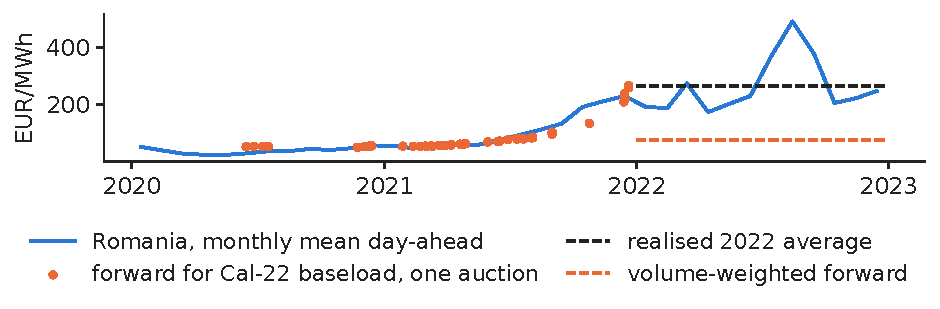
\includegraphics[width=\textwidth,height=0.525\textheight,keepaspectratio]{charts/en/crisis_cal22.pdf}\end{center}\vspace{-3mm}
\chartsource{Source: OPCOM (PCCB-LE-flex results; day-ahead prices via energy-charts.info); ECB. Data: 150 auctions for 2022 baseload; spot 2020-2022.}
\vspace{0.5mm}
\begin{itemize}\setlength{\itemsep}{0pt}
  \item 2022 baseload: 150 auctions, volume-weighted average price (VWAP) 77.4 EUR/MWh; spot 265.3
    \begin{itemize}\setlength{\itemsep}{0pt}
      \item 2020: 54.4; first half of 2021: 61.5; second half: 136.7; saving 1.65 million EUR per MW
    \end{itemize}
\end{itemize}
\par\vfill\manager{when you hedge matters: contracts bought late in 2021 cost twice as much.}\par\vspace{0.5mm}
\par\vfill\noindent{\scriptsize\color{FooterGray}(own computation; OPCOM)}\hfill\qlink{EMQA\_L5\_crisis\_cal22}{Quantlets/L5/EMQA_L5_crisis_cal22}\par\vspace{0.5mm}
\end{frame}

\begin{frame}{The crisis froze forward trading and brought regulated prices}
\footnotesize
\begin{itemize}\setlength{\itemsep}{1pt}
  \item \textbf{A transfer, not a gain}
    \begin{itemize}\setlength{\itemsep}{0pt}
      \item Each MWh sold forward for 2022 went 187.9 EUR/MWh below spot: producers lost what hedged suppliers saved
    \end{itemize}
  \item \textbf{Then forwards overshot}
    \begin{itemize}\setlength{\itemsep}{0pt}
      \item Calendar 2023 traded up to 509.2 on 17 Aug 2022; 2023 averaged 103.7 EUR/MWh
    \end{itemize}
  \item \textbf{Romania}
    \begin{itemize}\setlength{\itemsep}{0pt}
      \item Government Emergency Ordinance (OUG) 27/2022: capped final prices
      \item OUG 153/2022: Centralised Electricity Purchase Mechanism (MACEE), OPCOM single buyer at 450 lei/MWh for 2023--2024
      \item OPCOM forward volume: 27.3 TWh in 2021, 1.6 TWh in 2023
    \end{itemize}
  \item \textbf{In the EU}
    \begin{itemize}\setlength{\itemsep}{0pt}
      \item The EU Agency for the Cooperation of Energy Regulators (ACER) kept the market design and flagged thin forward markets beyond three years
    \end{itemize}
\end{itemize}
\par\vfill\manager{write the hedging policy before the crisis
    \begin{itemize}\setlength{\itemsep}{0pt}
      \item During it, nobody can agree on one.
    \end{itemize}}\par\vspace{0.5mm}
\par\vfill\noindent{\scriptsize\color{FooterGray}(OUG 27/2022; OUG 153/2022; ACER, 2022; OPCOM)}\hfill\tryit{notebook \S2}\par\vspace{0.5mm}
\end{frame}


\section{Forwards, futures and the forward curve}

\subsection{Contracts}

\begin{frame}{A power forward delivers constant MW over a whole period}
\footnotesize
\intuition{A baseload forward fixes today the price of every hour of a month, quarter or year.}
\begin{columns}[T,onlytextwidth]
\begin{column}{0.53\textwidth}
\[ \bar S=\frac{1}{H}\sum_{h=1}^{H}S_h,\qquad \underbrace{V_T=q\,H\,(\bar S-F)}_{\text{value to the buyer}} \]{\footnotesize\begin{itemize}\setlength{\itemsep}{0pt}
  \item \textbf{\txtwhere}
    \begin{itemize}\setlength{\itemsep}{0pt}
      \item $H$ = hours of the delivery period (744 in a 31-day month, 8\,760 in a year)
      \item $S_h$ = day-ahead price of hour $h$
      \item $q$ = power, MW
      \item $F$ = forward price.
    \end{itemize}
\end{itemize}\par}
\end{column}
\begin{column}{0.44\textwidth}
\begin{itemize}\setlength{\itemsep}{1pt}
  \item \textbf{Profiles}
    \begin{itemize}\setlength{\itemsep}{0pt}
      \item Band: all hours, Monday to Sunday (LD), 94\% of volume
      \item Peak: the peak hours of working days only
    \end{itemize}
  \item \textbf{OPCOM, 31 Oct 2026}
    \begin{itemize}\setlength{\itemsep}{0pt}
      \item Year 2027: 148.1 EUR/MWh $\times$ 8\,760 MWh per MW
      \item Next month: 215.3 EUR/MWh
    \end{itemize}
\end{itemize}
\end{column}
\end{columns}
\par\vfill\manager{price a customer's contract on the forward of its delivery period, not on today's spot.}\par\vspace{0.5mm}
\par\vfill\noindent{\scriptsize\color{FooterGray}(OPCOM; Benth et al., 2008)}\hfill\tryit{notebook \S3}\par\vspace{0.5mm}
\end{frame}

\begin{frame}{Physical delivery and cash settlement}
\footnotesize
\intuition{A physical forward delivers MWh at $F$; a cash-settled future pays the gap to a reference average.}
\begin{columns}[T,onlytextwidth]
\begin{column}{0.55\textwidth}
\[ \underbrace{F\cdot Q}_{\text{physical}}=\underbrace{\bar S Q}_{\text{spot}}-\underbrace{(\bar S^{\text{ref}}-F)Q}_{\text{cash settlement}}\ \text{only if } \bar S^{\text{ref}}=\bar S \]{\footnotesize\begin{itemize}\setlength{\itemsep}{0pt}
  \item \textbf{\txtwhere}
    \begin{itemize}\setlength{\itemsep}{0pt}
      \item $\bar S^{\text{ref}}$ = settlement index of the future (e.g.\ the German average)
      \item Otherwise the gap is basis risk (section 4).
    \end{itemize}
\end{itemize}\par}
\end{column}
\begin{column}{0.42\textwidth}
\begin{itemize}\setlength{\itemsep}{1pt}
  \item \textbf{Physical, Romania}
    \begin{itemize}\setlength{\itemsep}{0pt}
      \item OPCOM PCCB-LE auctions and continuous trading of standard contracts (PC-OTC)
      \item No basis risk
    \end{itemize}
  \item \textbf{Cash-settled, abroad}
    \begin{itemize}\setlength{\itemsep}{0pt}
      \item EEX and HUDEX futures, cleared
      \item Margin calls replace counterparty risk
    \end{itemize}
\end{itemize}
\end{column}
\end{columns}
\par\vfill\manager{physical when you need MWh in Romania
    \begin{itemize}\setlength{\itemsep}{0pt}
      \item Cash-settled when you need liquidity and can carry the basis.
    \end{itemize}}\par\vspace{0.5mm}
\par\vfill\noindent{\scriptsize\color{FooterGray}(OPCOM; Hull, 2022)}\par\vspace{0.5mm}
\end{frame}

\begin{frame}{Futures are marked to market daily: the hedge needs cash}
\footnotesize
\intuition{A forward settles once at delivery; a future pays or collects every day's price change.}
\begin{columns}[T,onlytextwidth]
\begin{column}{0.54\textwidth}
\[ \underbrace{VM_t=Q(F_t-F_{t-1})}_{\text{variation margin}},\qquad \sum_{t=1}^{T}VM_t=Q(F_T-F_0) \]{\footnotesize\begin{itemize}\setlength{\itemsep}{0pt}
  \item \textbf{\txtwhere}
    \begin{itemize}\setlength{\itemsep}{0pt}
      \item $F_t$ = settlement price of day $t$
      \item $Q$ = MWh
      \item Initial margin from a value-at-risk (VaR) model (Lecture 4).
    \end{itemize}
\end{itemize}\par}
\end{column}
\begin{column}{0.43\textwidth}
\begin{itemize}\setlength{\itemsep}{1pt}
  \item \textbf{NYMEX TTF, December 2026}
    \begin{itemize}\setlength{\itemsep}{0pt}
      \item 1\,487 daily prices, 15.1 -- 103.9 EUR/MWh
      \item Largest daily move 11.83 EUR/MWh, 29 Aug 2022
      \item 10 MW $\times$ 744 h: margin call 88\,015 EUR in a day
    \end{itemize}
\end{itemize}
\end{column}
\end{columns}
\par\vfill\manager{size a credit line for the worst daily move before hedging on an exchange.}\par\vspace{0.5mm}
\par\vfill\noindent{\scriptsize\color{FooterGray}(own computation; Hull, 2022)}\hfill\tryit{notebook \S3}\par\vspace{0.5mm}
\end{frame}

\begin{frame}{Romanian forward volume collapsed in 2022--2023}
\small
\begin{center}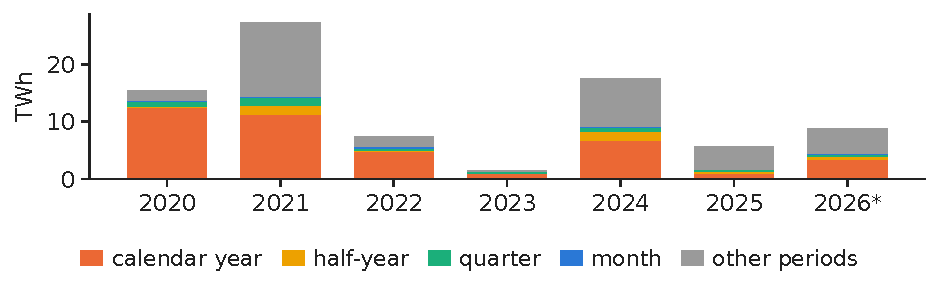
\includegraphics[width=\textwidth,height=0.526\textheight,keepaspectratio]{charts/en/fw_volume.pdf}\end{center}\vspace{-3mm}
\chartsource{Source: OPCOM, PCCB-LE-flex results; ECB (EUR/RON). Data: 2,298 traded auctions, 2020-05-12 to 2026-10-31; *2026 to the cut-off.}
\vspace{0.5mm}
\begin{itemize}\setlength{\itemsep}{0pt}
  \item Three producers sell 83\% of the volume: lignite 32\%, nuclear 30\%, hydro 21\%
    \begin{itemize}\setlength{\itemsep}{0pt}
      \item Calendar-year products: 80\% of baseload volume
    \end{itemize}
\end{itemize}
\par\vfill\manager{liquidity is thin: spread purchases over many auctions.}\par\vspace{0.5mm}
\par\vfill\noindent{\scriptsize\color{FooterGray}(own computation; OPCOM)}\hfill\qlink{EMQA\_L5\_fw\_volume}{Quantlets/L5/EMQA_L5_fw_volume}\par\vspace{0.5mm}
\end{frame}

\subsection{The forward curve}

\begin{frame}{Storable gas follows the cost of carry; power does not}
\footnotesize
\intuition{Gas can be stored, which ties forward to spot; power cannot, so its forward is an expectation plus a risk premium.}
\begin{columns}[T,onlytextwidth]
\begin{column}{0.52\textwidth}
\[ \underbrace{F_{t,T}=S_te^{(r+u-y)(T-t)}}_{\text{storable}},\qquad \underbrace{F_{t,T}=\E_t[\bar S_T]+\pi_{t,T}}_{\text{power}} \]{\footnotesize\begin{itemize}\setlength{\itemsep}{0pt}
  \item \textbf{\txtwhere}
    \begin{itemize}\setlength{\itemsep}{0pt}
      \item $r$ = interest rate
      \item $u$ = storage cost
      \item $y$ = convenience yield
      \item $\pi$ = risk premium
      \item Contango $F>S$, backwardation $F<S$.
    \end{itemize}
\end{itemize}\par}
\end{column}
\begin{column}{0.45\textwidth}
\begin{itemize}\setlength{\itemsep}{1pt}
  \item \textbf{Gas}, NYMEX TTF, 30 Oct 2026
    \begin{itemize}\setlength{\itemsep}{0pt}
      \item Dec 2026 103.9, May 2027 78.1 EUR/MWh
      \item Winter above summer pays for storage
    \end{itemize}
  \item \textbf{Power}, OPCOM
    \begin{itemize}\setlength{\itemsep}{0pt}
      \item October spot 239.3; Q1 2027 176.7; year 148.1
      \item Backwardation: the spike is expected to fade
    \end{itemize}
\end{itemize}
\end{column}
\end{columns}
\par\vfill\manager{never put today's spot into next year's budget
    \begin{itemize}\setlength{\itemsep}{0pt}
      \item Use the curve.
    \end{itemize}}\par\vspace{0.5mm}
\par\vfill\noindent{\scriptsize\color{FooterGray}(Fama \& French, 1987; Bessembinder \& Lemmon, 2002)}\hfill\tryit{notebook \S3}\par\vspace{0.5mm}
\end{frame}

\begin{frame}{The Romanian forward curve slopes down from a high spot}
\small
\begin{center}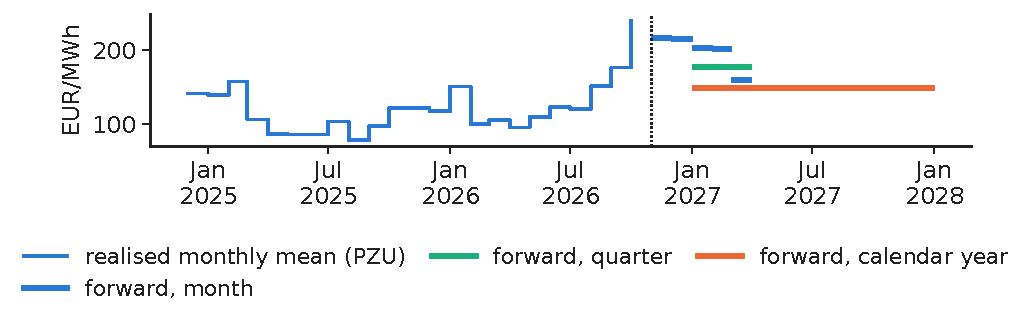
\includegraphics[width=\textwidth,height=0.537\textheight,keepaspectratio]{charts/en/fwd_curve.pdf}\end{center}\vspace{-3mm}
\chartsource{Source: OPCOM (PCCB-LE-flex results; day-ahead prices via energy-charts.info); ECB. Data: 85 auctions 2026-09-01 to 2026-10-31.}
\vspace{0.5mm}
\begin{itemize}\setlength{\itemsep}{0pt}
  \item 7 baseload products, VWAP per delivery period: next month 215.3, Q1 176.7, year 2027 148.1 EUR/MWh.
\end{itemize}
\par\vfill\manager{a 2027 offer starts from 148 EUR/MWh, not from the October spot.}\par\vspace{0.5mm}
\par\vfill\noindent{\scriptsize\color{FooterGray}(own computation; OPCOM)}\hfill\qlink{EMQA\_L5\_fwd\_curve}{Quantlets/L5/EMQA_L5_fwd_curve}\par\vspace{0.5mm}
\end{frame}

\begin{frame}{The curve moves: yearly forwards by trade date vs realised}
\small
\begin{center}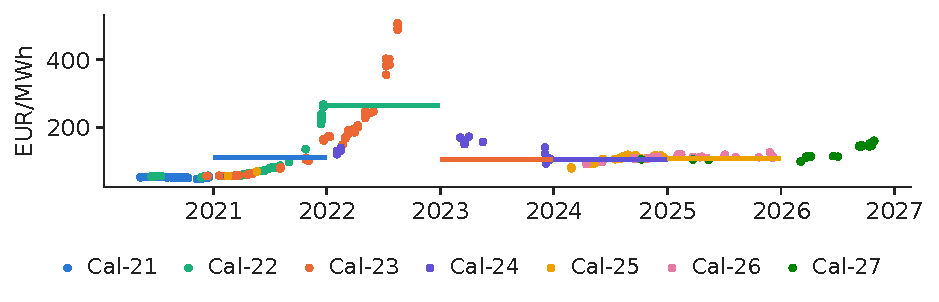
\includegraphics[width=\textwidth,height=0.485\textheight,keepaspectratio]{charts/en/cal_by_trade.pdf}\end{center}\vspace{-3mm}
\chartsource{Source: OPCOM (PCCB-LE-flex results; day-ahead prices via energy-charts.info); ECB. Data: calendar-year baseload auctions to 2026-10-31; thick line = realised mean.}
\vspace{0.5mm}
\begin{itemize}\setlength{\itemsep}{0pt}
  \item 2021: VWAP 51.3, realised 111.4
    \begin{itemize}\setlength{\itemsep}{0pt}
      \item 2023: 172.5 vs 103.7
      \item 2025: 102.1 vs 108.2 EUR/MWh.
    \end{itemize}
\end{itemize}
\par\vfill\manager{the forward is the price of certainty, not a forecast to rely on in a crisis.}\par\vspace{0.5mm}
\par\vfill\noindent{\scriptsize\color{FooterGray}(own computation; OPCOM)}\hfill\qlink{EMQA\_L5\_cal\_by\_trade}{Quantlets/L5/EMQA_L5_cal_by_trade}\par\vspace{0.5mm}
\end{frame}

\begin{frame}{The ex-post forward premium has no stable sign in Romania}
\footnotesize
\intuition{If buyers fear spikes more than sellers fear slumps, forwards trade above the expected spot.}
\begin{columns}[T,onlytextwidth]
\begin{column}{0.50\textwidth}
\[ \hat\pi_i=F_i-\bar S_i,\qquad t=\frac{\bar\pi}{\widehat{\text{se}}_{\text{HAC}}(\bar\pi)} \]{\footnotesize\begin{itemize}\setlength{\itemsep}{0pt}
  \item \textbf{\txtwhere}
    \begin{itemize}\setlength{\itemsep}{0pt}
      \item $i$ = delivery month
      \item $F_i$ = VWAP of the monthly band bought the month before
      \item $\bar S_i$ = realised mean
      \item Standard error heteroskedasticity- and autocorrelation-consistent (HAC), Newey--West, 3 lags.
    \end{itemize}
\end{itemize}\par}
\end{column}
\begin{column}{0.47\textwidth}
\begin{itemize}\setlength{\itemsep}{1pt}
  \item \textbf{One month ahead}, 30 months
    \begin{itemize}\setlength{\itemsep}{0pt}
      \item Mean \ensuremath{+}5.2 EUR/MWh, $t$ = 0.42, $p$ = 0.68
      \item Since 2023: \ensuremath{+}24.5, $t$ = 1.51
    \end{itemize}
  \item \textbf{All products}, volume-weighted
    \begin{itemize}\setlength{\itemsep}{0pt}
      \item Delivered to 2021: \ensuremath{-}55.8
      \item 2022: \ensuremath{-}166.5; from 2023: \ensuremath{+}29.7 EUR/MWh
    \end{itemize}
\end{itemize}
\end{column}
\end{columns}
\par\vfill\manager{hedging is cheap on average
    \begin{itemize}\setlength{\itemsep}{0pt}
      \item Its real cost is the upside you give up.
    \end{itemize}}\par\vspace{0.5mm}
\par\vfill\noindent{\scriptsize\color{FooterGray}(Bessembinder \& Lemmon, 2002; Redl et al., 2009)}\hfill\tryit{notebook \S3}\par\vspace{0.5mm}
\end{frame}

\begin{frame}{Month by month, forward minus spot swings both ways}
\small
\begin{center}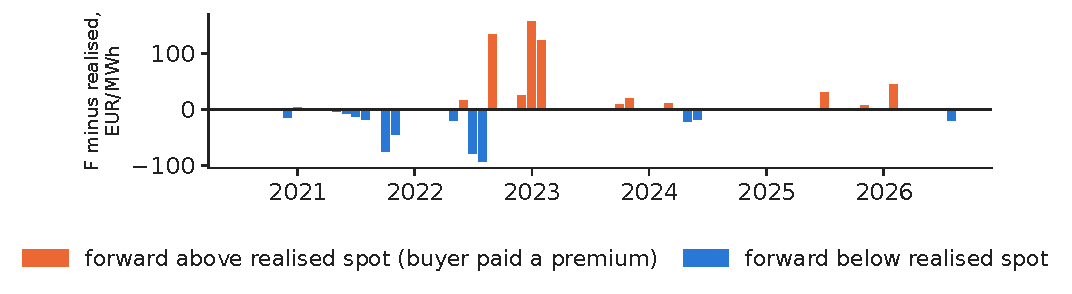
\includegraphics[width=\textwidth,height=0.530\textheight,keepaspectratio]{charts/en/premium.pdf}\end{center}\vspace{-3mm}
\chartsource{Source: OPCOM (PCCB-LE-flex results; day-ahead prices via energy-charts.info); ECB. Data: 30 delivery months, 2020-08 to 2026-08.}
\vspace{0.5mm}
\begin{itemize}\setlength{\itemsep}{0pt}
  \item Median \ensuremath{-}0.2 EUR/MWh
    \begin{itemize}\setlength{\itemsep}{0pt}
      \item The deep negative bars are 2021--2022 surprises, not a stable discount.
    \end{itemize}
\end{itemize}
\par\vfill\manager{judge a hedge by the risk it removed, not by its ex-post profit.}\par\vspace{0.5mm}
\par\vfill\noindent{\scriptsize\color{FooterGray}(own computation; OPCOM)}\hfill\qlink{EMQA\_L5\_premium}{Quantlets/L5/EMQA_L5_premium}\par\vspace{0.5mm}
\end{frame}


\section{Spreads: the margins of power plants}

\begin{frame}{Clean spark spread: power minus gas minus carbon}
\footnotesize
\intuition{A gas plant sells 1 MWh of power, burns $1/\eta$ MWh of gas and pays for its CO$_2$.}
\begin{columns}[T,onlytextwidth]
\begin{column}{0.55\textwidth}
\[ SS=P-\frac{G}{\eta_g},\qquad CSS=P-\frac{G}{\eta_g}-\frac{e_g}{\eta_g}A \]{\footnotesize\begin{itemize}\setlength{\itemsep}{0pt}
  \item \textbf{\txtwhere}
    \begin{itemize}\setlength{\itemsep}{0pt}
      \item Spark spread (SS), clean spark spread (CSS)
      \item $P$ = power, EUR/MWh
      \item $G$ = gas, EUR/MWh thermal
      \item $\eta_g$ = efficiency of the gas plant, 0.50 (assumed)
      \item $e_g$ = emission factor of gas, 0.202 t CO$_2$/MWh thermal, Intergovernmental Panel on Climate Change (IPCC)
      \item $A$ = EUA, EUR/t.
    \end{itemize}
\end{itemize}\par}
\end{column}
\begin{column}{0.42\textwidth}
\begin{itemize}\setlength{\itemsep}{1pt}
  \item \textbf{Romania, Oct 2026}
    \begin{itemize}\setlength{\itemsep}{0pt}
      \item Power 239.3; gas cost per MWh of power 173.6 (= 86.8/0.5); carbon 33.3
      \item SS \ensuremath{+}65.7, CSS \ensuremath{+}32.4 EUR/MWh
    \end{itemize}
  \item \textbf{Yearly mean CSS}
    \begin{itemize}\setlength{\itemsep}{0pt}
      \item Romania: 2022 \ensuremath{-}32.2, 2025 \ensuremath{+}5.8
      \item Germany: 2022 \ensuremath{-}62.2, 2025 \ensuremath{-}13.1
    \end{itemize}
\end{itemize}
\end{column}
\end{columns}
\par\vfill\manager{a gas producer hedges the spread: sell power, buy gas and EUA forward together.}\par\vspace{0.5mm}
\par\vfill\noindent{\scriptsize\color{FooterGray}(IPCC, 2006; Deng et al., 2001)}\hfill\tryit{notebook \S4}\par\vspace{0.5mm}
\end{frame}

\begin{frame}{Dark spreads and the carbon price that favours gas over coal}
\footnotesize
\intuition{Coal emits more CO$_2$ per MWh, so a high EUA price pushes coal behind gas in the merit order.}
\begin{columns}[T,onlytextwidth]
\begin{column}{0.56\textwidth}
\[ CDS=P-\frac{C}{\eta_c}-\frac{e_c}{\eta_c}A,\qquad A^{*}=\frac{G/\eta_g-C/\eta_c}{e_c/\eta_c-e_g/\eta_g} \]{\footnotesize\begin{itemize}\setlength{\itemsep}{0pt}
  \item \textbf{\txtwhere}
    \begin{itemize}\setlength{\itemsep}{0pt}
      \item Clean dark spread (CDS)
      \item $C$ = coal price, EUR/MWh thermal (USD/t $\div$ EUR/USD $\div$ 6.978)
      \item $\eta_c$ = coal plant efficiency, 0.38 (assumed)
      \item $e_c$ = emission factor, 0.341 t CO$_2$/MWh thermal
      \item $A^{*}$ = EUA price at which CSS = CDS.
    \end{itemize}
\end{itemize}\par}
\end{column}
\begin{column}{0.41\textwidth}
\begin{itemize}\setlength{\itemsep}{1pt}
  \item \textbf{Month: Oct 2026}
    \begin{itemize}\setlength{\itemsep}{0pt}
      \item Coal 12.8 EUR/MWh thermal; CDS Romania \ensuremath{+}131.7
      \item $A^{*}$ = 283.7 EUR/t vs EUA 82.4
    \end{itemize}
  \item \textbf{Caveats}
    \begin{itemize}\setlength{\itemsep}{0pt}
      \item Lignite has no market price; coal = South African export price
      \item EUA = EEX auctions, then the ETC from Jan 2026
    \end{itemize}
\end{itemize}
\end{column}
\end{columns}
\par\vfill\manager{a coal producer selling power forward should buy EUA forward with it.}\par\vspace{0.5mm}
\par\vfill\noindent{\scriptsize\color{FooterGray}(IPCC, 2006; World Bank)}\hfill\tryit{notebook \S4}\par\vspace{0.5mm}
\end{frame}

\begin{frame}{Monthly clean spark and clean dark spreads}
\small
\begin{center}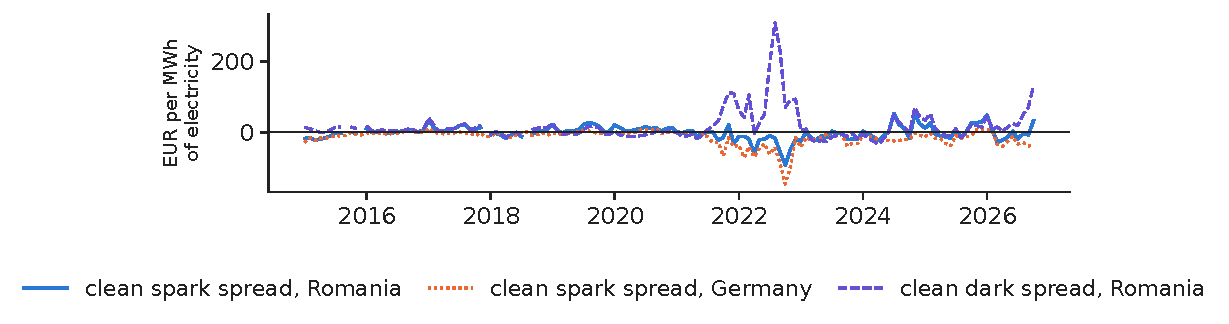
\includegraphics[width=\textwidth,height=0.562\textheight,keepaspectratio]{charts/en/spreads.pdf}\end{center}\vspace{-3mm}
\chartsource{Source: energy-charts.info; World Bank (TTF, coal); EEX and SparkChange ETC (EUA); ECB. Data: monthly, 2015-01 to 2026-10.}
\vspace{0.5mm}
\begin{itemize}\setlength{\itemsep}{0pt}
  \item CSS negative in 67 of 138 months in Romania, 121 in Germany
    \begin{itemize}\setlength{\itemsep}{0pt}
      \item Romania higher by 13.9 EUR/MWh on average.
    \end{itemize}
\end{itemize}
\par\vfill\manager{a mean spread near zero does not make a plant worthless: it runs only in good hours.}\par\vspace{0.5mm}
\par\vfill\noindent{\scriptsize\color{FooterGray}(own computation; IPCC, 2006)}\hfill\qlink{EMQA\_L5\_spreads}{Quantlets/L5/EMQA_L5_spreads}\par\vspace{0.5mm}
\end{frame}

\begin{frame}{A flexible gas plant is a strip of hourly call options}
\footnotesize
\intuition{The plant runs only when the spread is positive, so it earns the positive part of each hourly spread.}
\begin{columns}[T,onlytextwidth]
\begin{column}{0.52\textwidth}
\[ \underbrace{\sum_h \max(CSS_h,0)}_{\text{flexible}}\ \ge\ \max\Big(\underbrace{\sum_h CSS_h}_{\text{must-run}},0\Big) \]{\footnotesize\begin{itemize}\setlength{\itemsep}{0pt}
  \item \textbf{\txtwhere}
    \begin{itemize}\setlength{\itemsep}{0pt}
      \item $CSS_h$ = clean spark spread of hour $h$, 1 MW, gas and EUA at monthly means
      \item No start-up costs, so an upper bound.
    \end{itemize}
\end{itemize}\par}
\end{column}
\begin{column}{0.45\textwidth}
\begin{itemize}\setlength{\itemsep}{1pt}
  \item \textbf{Romania}, last 12 months
    \begin{itemize}\setlength{\itemsep}{0pt}
      \item Positive in 58\% of hours
      \item Must-run 38\,095, flexible 235\,494 EUR per MW
    \end{itemize}
  \item \textbf{Germany}
    \begin{itemize}\setlength{\itemsep}{0pt}
      \item Positive in 41\% of hours
      \item Must-run \ensuremath{-}165\,206, flexible 112\,724 EUR per MW
    \end{itemize}
\end{itemize}
\end{column}
\end{columns}
\par\vfill\manager{value a gas plant or a battery as options, never as a mean spread times 8\,760 h.}\par\vspace{0.5mm}
\par\vfill\noindent{\scriptsize\color{FooterGray}(Deng et al., 2001; Eydeland \& Wolyniec, 2003)}\hfill\tryit{notebook \S4}\par\vspace{0.5mm}
\end{frame}

\begin{frame}{Sorted hourly spreads: the value lies in the best hours}
\small
\begin{center}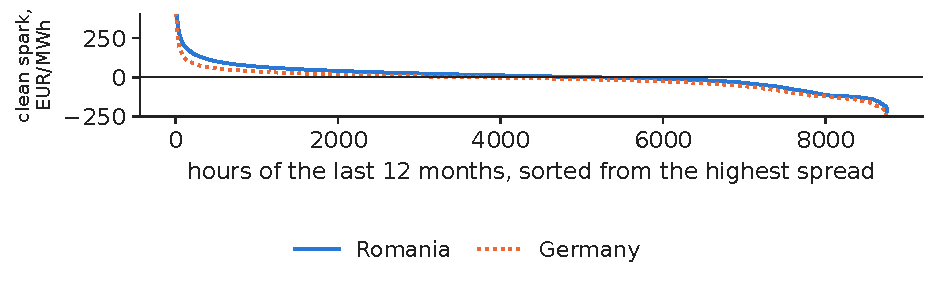
\includegraphics[width=\textwidth,height=0.529\textheight,keepaspectratio]{charts/en/spark_hourly.pdf}\end{center}\vspace{-3mm}
\chartsource{Source: energy-charts.info; World Bank (TTF, coal); EEX and SparkChange ETC (EUA); ECB. Data: 2025-11-01 to 2026-10-31, hourly.}
\vspace{0.5mm}
\begin{itemize}\setlength{\itemsep}{0pt}
  \item The area above zero is the option value
    \begin{itemize}\setlength{\itemsep}{0pt}
      \item At equal gas and carbon prices Romania has more profitable hours than Germany.
    \end{itemize}
\end{itemize}
\par\vfill\manager{hedge a flexible plant with peak products, not with a band.}\par\vspace{0.5mm}
\par\vfill\noindent{\scriptsize\color{FooterGray}(own computation)}\hfill\qlink{EMQA\_L5\_spark\_hourly}{Quantlets/L5/EMQA_L5_spark_hourly}\par\vspace{0.5mm}
\end{frame}


\section{Hedge ratio, basis risk and shape risk}

\begin{frame}{The minimum-variance hedge ratio is a regression slope}
\footnotesize
\intuition{Choose the contracts per MWh of exposure that make the hedged cost vary least.}
\begin{columns}[T,onlytextwidth]
\begin{column}{0.58\textwidth}
\[ h^{*}=\arg\min_h\Var(\Delta S-h\Delta F)=\rho\frac{\sigma_S}{\sigma_F}=\frac{\Cov(\Delta S,\Delta F)}{\Var(\Delta F)} \]\[ \Delta S_t=a+h\,\Delta F_t+\varepsilon_t,\qquad HE=\rho^2 \]{\footnotesize\begin{itemize}\setlength{\itemsep}{0pt}
  \item \textbf{\txtwhere}
    \begin{itemize}\setlength{\itemsep}{0pt}
      \item $\Delta S$, $\Delta F$ = monthly changes of the exposure and of the hedge
      \item $\rho$ = their correlation
      \item Hedge effectiveness (HE) = variance removed
      \item $h^{*}$ by ordinary least squares (OLS)
      \item Derivation in Appendix A.
    \end{itemize}
\end{itemize}\par}
\end{column}
\begin{column}{0.39\textwidth}
\begin{itemize}\setlength{\itemsep}{1pt}
  \item \textbf{Instrument}
    \begin{itemize}\setlength{\itemsep}{0pt}
      \item A cash-settled future ends at its zone's monthly mean: we use HU and DE-LU means
      \item 133 months, Feb 2015 -- Oct 2026
    \end{itemize}
  \item \textbf{Uncertainty}
    \begin{itemize}\setlength{\itemsep}{0pt}
      \item HAC standard error, 3 lags
      \item Block bootstrap, 6-month blocks, 2\,000 draws
    \end{itemize}
\end{itemize}
\end{column}
\end{columns}
\par\vfill\manager{a hedge ratio without a confidence interval is a guess.}\par\vspace{0.5mm}
\par\vfill\noindent{\scriptsize\color{FooterGray}(Johnson, 1960; Ederington, 1979)}\hfill\tryit{notebook \S5}\par\vspace{0.5mm}
\end{frame}

\begin{frame}{Hungary hedges Romania almost fully; Germany leaves a fifth}
\footnotesize
\begin{center}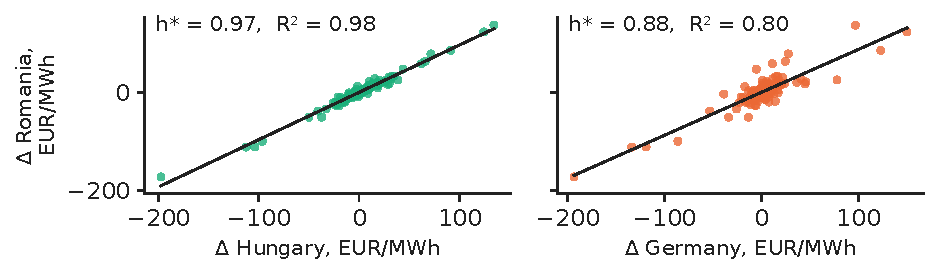
\includegraphics[width=\textwidth,height=0.449\textheight,keepaspectratio]{charts/en/hedge_scatter.pdf}\end{center}\vspace{-3mm}
\chartsource{Source: energy-charts.info: day-ahead prices of OPCOM, HUPX, EPEX SPOT. Data: monthly changes, 2015-02 to 2026-10.}
\vspace{0.3mm}
\begin{center}{\scriptsize\renewcommand{\arraystretch}{1.05}\setlength{\tabcolsep}{4pt}
\begin{tabular}{@{}lrrrrrr@{}}\toprule
Hedge & $h^{*}$ & HAC s.e. & bootstrap 95\% & $R^2$ & $h^{*}$ 2015--20 & variance cut from 2021 \\ \midrule
Hungary & 0.966 & 0.023 & [0.93; 1.03] & 0.98 & 0.92 & 97.9\% \\
Germany & 0.875 & 0.049 & [0.73; 1.01] & 0.80 & 0.91 & 81.1\% \\
\bottomrule\end{tabular}}\end{center}
\par\vfill\manager{hedge with Hungarian futures before German ones.}\par\vspace{0.5mm}
\par\vfill\noindent{\scriptsize\color{FooterGray}(own computation; out of sample: $h^{*}$ of 2015--2020 applied from 2021)}\hfill\qlink{EMQA\_L5\_hedge\_scatter}{Quantlets/L5/EMQA_L5_hedge_scatter}\par\vspace{0.5mm}
\end{frame}

\begin{frame}{Basis risk: what a foreign hedge leaves behind}
\footnotesize
\intuition{Hedged with a German future, a Romanian supplier pays the German forward plus the Romania--Germany gap at delivery.}
\begin{columns}[T,onlytextwidth]
\begin{column}{0.55\textwidth}
\[ \bar S^{\text{RO}}-h(\bar S^{X}-F^{X}_0)=hF^{X}_0+\underbrace{(\bar S^{\text{RO}}-h\bar S^{X})}_{\text{basis } b} \]{\footnotesize\begin{itemize}\setlength{\itemsep}{0pt}
  \item \textbf{\txtwhere}
    \begin{itemize}\setlength{\itemsep}{0pt}
      \item $X$ = zone of the future (HU, DE-LU)
      \item $F^{X}_0$ = its price today
      \item With $h=1$, $b$ = monthly price gap Romania minus $X$.
    \end{itemize}
\end{itemize}\par}
\end{column}
\begin{column}{0.42\textwidth}
\begin{itemize}\setlength{\itemsep}{1pt}
  \item \textbf{Romania -- Hungary}
    \begin{itemize}\setlength{\itemsep}{0pt}
      \item Mean \ensuremath{-}2.1, st.\ dev.\ 4.5 EUR/MWh
      \item Equal prices in 56\% of hours in 2021
    \end{itemize}
  \item \textbf{Romania -- Germany}
    \begin{itemize}\setlength{\itemsep}{0pt}
      \item Mean \ensuremath{+}13.9, st.\ dev.\ 15.2
      \item Since 2023 mean \ensuremath{+}18.7 EUR/MWh
    \end{itemize}
\end{itemize}
\end{column}
\end{columns}
\par\vfill\manager{a German hedge costs the German forward plus about 19 EUR/MWh: price it in.}\par\vspace{0.5mm}
\par\vfill\noindent{\scriptsize\color{FooterGray}(Hull, 2022; own computation)}\hfill\tryit{notebook \S5}\par\vspace{0.5mm}
\end{frame}

\begin{frame}{The basis became more volatile after 2021, though RO and HU often share a price}
\small
\begin{center}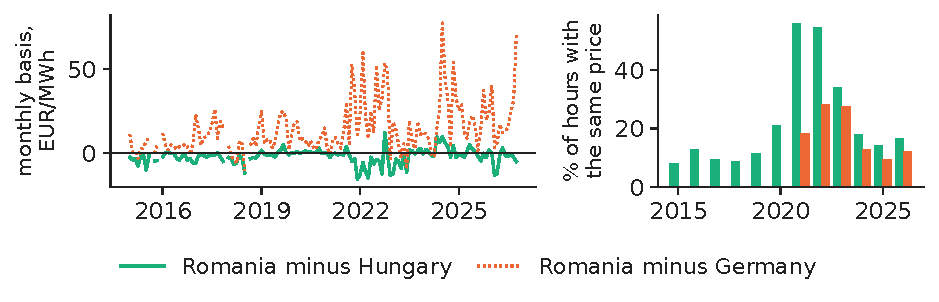
\includegraphics[width=\textwidth,height=0.466\textheight,keepaspectratio]{charts/en/basis.pdf}\end{center}\vspace{-3mm}
\chartsource{Source: energy-charts.info: day-ahead prices of OPCOM, HUPX, EPEX SPOT. Data: 2015-01 to 2026-10; right: |difference| < 0.01 EUR/MWh.}
\vspace{0.5mm}
\begin{itemize}\setlength{\itemsep}{0pt}
  \item Basis to Germany, st.\ dev.\ 7.6 before 2021 and 18.2 after
    \begin{itemize}\setlength{\itemsep}{0pt}
      \item Coupling steps: 17 June 2021 (Interim Coupling), 8 June 2022 (Core flow-based).
    \end{itemize}
\end{itemize}
\par\vfill\manager{prices converge only without congestion: basis risk is congestion risk.}\par\vspace{0.5mm}
\par\vfill\noindent{\scriptsize\color{FooterGray}(own computation; ENTSO-E, 2021)}\hfill\qlink{EMQA\_L5\_basis}{Quantlets/L5/EMQA_L5_basis}\par\vspace{0.5mm}
\end{frame}

\begin{frame}{Shape risk: customers do not consume a flat band}
\footnotesize
\intuition{A band covers the same MW every hour; load is higher in dear hours, solar output in cheap ones.}
\begin{columns}[T,onlytextwidth]
\begin{column}{0.53\textwidth}
\[ f^{\text{load}}=\frac{\sum_h L_hP_h}{\bar P\sum_h L_h},\qquad f^{\text{solar}}=\frac{\sum_h Q_hP_h}{\bar P\sum_h Q_h} \]{\footnotesize\begin{itemize}\setlength{\itemsep}{0pt}
  \item \textbf{\txtwhere}
    \begin{itemize}\setlength{\itemsep}{0pt}
      \item $L_h$ = Romanian load, $Q_h$ = solar output in hour $h$
      \item $\bar P$ = simple mean price of the year
      \item $f>1$: the profile costs more than the band.
    \end{itemize}
\end{itemize}\par}
\end{column}
\begin{column}{0.44\textwidth}
\begin{itemize}\setlength{\itemsep}{1pt}
  \item \textbf{Supplier}, national load
    \begin{itemize}\setlength{\itemsep}{0pt}
      \item $f^{\text{load}}$: 1.039 (2019), 1.066 (2025)
      \item +7.1 EUR/MWh over the band in 2025
    \end{itemize}
  \item \textbf{Solar producer}
    \begin{itemize}\setlength{\itemsep}{0pt}
      \item $f^{\text{solar}}$: 1.045 (2019), 0.596 (2025)
      \item $-$43.7 EUR/MWh under the band in 2025
    \end{itemize}
\end{itemize}
\end{column}
\end{columns}
\par\vfill\manager{price a solar power purchase agreement (PPA) at the capture factor, not at the band forward.}\par\vspace{0.5mm}
\par\vfill\noindent{\scriptsize\color{FooterGray}(own computation)}\hfill\tryit{notebook \S5}\par\vspace{0.5mm}
\end{frame}

\begin{frame}{Value of the solar and load profiles relative to baseload}
\small
\begin{center}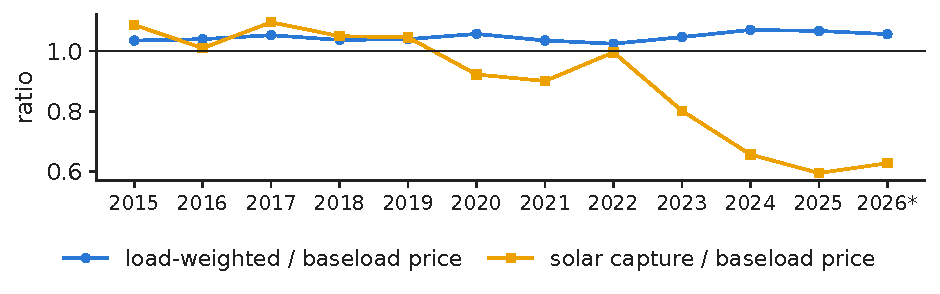
\includegraphics[width=\textwidth,height=0.562\textheight,keepaspectratio]{charts/en/shape.pdf}\end{center}\vspace{-3mm}
\chartsource{Source: energy-charts.info: OPCOM prices; ENTSO-E load and solar output. Data: hourly, 2015 to 2026-10-31; *to the cut-off.}
\vspace{0.5mm}
\begin{itemize}\setlength{\itemsep}{0pt}
  \item Solar capture factor down to 0.596 in 2025
    \begin{itemize}\setlength{\itemsep}{0pt}
      \item Load-weighted price 7.1 EUR/MWh above the band in 2025.
    \end{itemize}
\end{itemize}
\par\vfill\manager{buy band for the base of the portfolio, peak and hourly products for the shape.}\par\vspace{0.5mm}
\par\vfill\noindent{\scriptsize\color{FooterGray}(own computation)}\hfill\qlink{EMQA\_L5\_shape}{Quantlets/L5/EMQA_L5_shape}\par\vspace{0.5mm}
\end{frame}


\section{Options on energy}

\begin{frame}{Caps, floors and collars}
\footnotesize
\intuition{A call caps the purchase price and keeps the gain if prices fall; it costs a premium today.}
\begin{columns}[T,onlytextwidth]
\begin{column}{0.56\textwidth}
\[ \underbrace{(F_T-K)^+}_{\text{call}},\quad \underbrace{(K-F_T)^+}_{\text{put}},\quad \underbrace{\min(F_T,K_c)+c}_{\text{price with a cap}} \]\[ \text{collar: } \max\big(K_p,\min(F_T,K_c)\big)+c-p \]{\footnotesize\begin{itemize}\setlength{\itemsep}{0pt}
  \item \textbf{\txtwhere}
    \begin{itemize}\setlength{\itemsep}{0pt}
      \item $F_T$ = forward price at expiry $T$
      \item $K$ = strike
      \item $c$, $p$ = call and put premiums
      \item Collar = buy a call at $K_c$, sell a put at $K_p<K_c$.
    \end{itemize}
\end{itemize}\par}
\end{column}
\begin{column}{0.41\textwidth}
\begin{itemize}\setlength{\itemsep}{1pt}
  \item \textbf{Who uses what}
    \begin{itemize}\setlength{\itemsep}{0pt}
      \item Supplier: a cap (call)
      \item Producer: a floor (put)
      \item Both: a low-cost collar (the supplier buys a call and sells a put; the producer the reverse)
    \end{itemize}
  \item \textbf{In Romania}
    \begin{itemize}\setlength{\itemsep}{0pt}
      \item No listed power options
      \item Caps sit inside bilateral and PPA contracts
    \end{itemize}
\end{itemize}
\end{column}
\end{columns}
\par\vfill\manager{buy a cap when a spike would break the firm, not when it would merely hurt.}\par\vspace{0.5mm}
\par\vfill\noindent{\scriptsize\color{FooterGray}(Hull, 2022)}\hfill\tryit{notebook \S6}\par\vspace{0.5mm}
\end{frame}

\begin{frame}{Black-76 prices an option on a forward from five inputs}
\footnotesize
\intuition{Under the pricing measure a forward has no drift, so the option depends only on $F$, $K$, $T$, $r$ and $\sigma$.}
\begin{columns}[T,onlytextwidth]
\begin{column}{0.58\textwidth}
\[ C=e^{-rT}[F\Phi(d_1)-K\Phi(d_2)],\quad P=e^{-rT}[K\Phi(-d_2)-F\Phi(-d_1)] \]\[ d_1=\frac{\ln(F/K)+\sigma^2T/2}{\sigma\sqrt T},\qquad d_2=d_1-\sigma\sqrt T \]{\footnotesize\begin{itemize}\setlength{\itemsep}{0pt}
  \item \textbf{\txtwhere}
    \begin{itemize}\setlength{\itemsep}{0pt}
      \item $\Phi$ = standard normal distribution function
      \item $\sigma$ = annual volatility of $\ln F$
      \item $T$ in years
      \item $r$ = continuous rate (Appendix B).
    \end{itemize}
\end{itemize}\par}
\end{column}
\begin{column}{0.39\textwidth}
\begin{itemize}\setlength{\itemsep}{1pt}
  \item \textbf{Inputs}, 2027 band
    \begin{itemize}\setlength{\itemsep}{0pt}
      \item $F$ = 148.12 EUR/MWh (OPCOM VWAP)
      \item $T$ = 45 days; $r$ = 2.44\% (€STR)
      \item $\sigma$ = 0.220 (next slide)
    \end{itemize}
  \item \textbf{Prices}, EUR/MWh
    \begin{itemize}\setlength{\itemsep}{0pt}
      \item $K=F$: call = put = 4.55
      \item Cap at 1.1 $F$: 0.63
      \item Floor at 0.9 $F$: 0.43
    \end{itemize}
\end{itemize}
\end{column}
\end{columns}
\par\vfill\manager{ask the bank which volatility it used
    \begin{itemize}\setlength{\itemsep}{0pt}
      \item The premium grows almost linearly with $\sigma$.
    \end{itemize}}\par\vspace{0.5mm}
\par\vfill\noindent{\scriptsize\color{FooterGray}(Black, 1976; Hull, 2022)}\hfill\tryit{notebook \S6}\par\vspace{0.5mm}
\end{frame}

\begin{frame}{Volatility is the input you must estimate; real estimates disagree}
\footnotesize
\begin{columns}[T,onlytextwidth]
\begin{column}{0.55\textwidth}
\begin{itemize}\setlength{\itemsep}{1pt}
  \item \textbf{1. Romanian yearly forwards}
    \begin{itemize}\setlength{\itemsep}{0pt}
      \item Irregular auctions: $\hat\sigma^2=\sum_k(\Delta\ln F_k)^2/\sum_k\Delta t_k$, gaps $\le$ 30 days
      \item $\hat\sigma$ = 0.220 on 49 pairs of auction days
    \end{itemize}
  \item \textbf{2. TTF future, January 2027}
    \begin{itemize}\setlength{\itemsep}{0pt}
      \item Last 60 trading days: $\hat\sigma$ = 0.499; call 10.30
    \end{itemize}
  \item \textbf{3. Month average vs forward}
    \begin{itemize}\setlength{\itemsep}{0pt}
      \item $\text{sd}(\ln(\bar S/F)/\sqrt T)$ = 0.668, 153 auctions
    \end{itemize}
\end{itemize}
\end{column}
\begin{column}{0.42\textwidth}
\begin{itemize}\setlength{\itemsep}{1pt}
  \item \textbf{Why they differ}
    \begin{itemize}\setlength{\itemsep}{0pt}
      \item A year averages 8\,760 hours, far calmer than a month
      \item Gas has its own crisis in 2026
      \item No free implied volatility for Romania
    \end{itemize}
  \item \textbf{Better}
    \begin{itemize}\setlength{\itemsep}{0pt}
      \item Generalised autoregressive conditional heteroskedasticity (GARCH) models of Lecture 3
    \end{itemize}
\end{itemize}
\end{column}
\end{columns}
\par\vfill\manager{match the volatility to the underlying: year, quarter or month.}\par\vspace{0.5mm}
\par\vfill\noindent{\scriptsize\color{FooterGray}(own computation; OPCOM; Yahoo Finance)}\hfill\tryit{notebook \S6}\par\vspace{0.5mm}
\end{frame}

\begin{frame}{Near contracts move more: the Samuelson effect in TTF}
\small
\begin{center}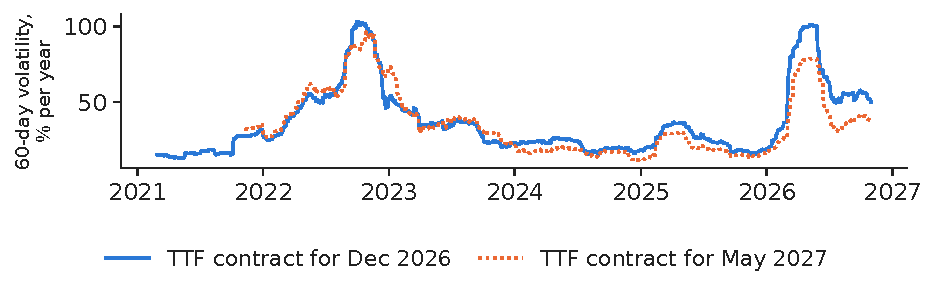
\includegraphics[width=\textwidth,height=0.568\textheight,keepaspectratio]{charts/en/samuelson.pdf}\end{center}\vspace{-3mm}
\chartsource{Source: Yahoo Finance, NYMEX TTF futures. Data: daily closes to 2026-10-31, rolling 60 trading days.}
\vspace{0.5mm}
\begin{itemize}\setlength{\itemsep}{0pt}
  \item 1 Nov 2025 -- 31 Oct 2026: December 2026 63\%, May 2027 48\% a year
    \begin{itemize}\setlength{\itemsep}{0pt}
      \item In 2022 both near 66\%.
    \end{itemize}
\end{itemize}
\par\vfill\manager{an option close to delivery needs a higher volatility.}\par\vspace{0.5mm}
\par\vfill\noindent{\scriptsize\color{FooterGray}(own computation; Samuelson, 1965)}\hfill\qlink{EMQA\_L5\_samuelson}{Quantlets/L5/EMQA_L5_samuelson}\par\vspace{0.5mm}
\end{frame}

\begin{frame}{Delta and vega: the option in MWh, and its volatility risk}
\footnotesize
\intuition{Delta is the forward quantity that offsets the option; vega is the premium change per volatility point.}
\begin{columns}[T,onlytextwidth]
\begin{column}{0.52\textwidth}
\[ \Delta_C=e^{-rT}\Phi(d_1),\quad \Delta_P=-e^{-rT}\Phi(-d_1) \]\[ \mathcal V=e^{-rT}F\varphi(d_1)\sqrt T,\qquad C-P=e^{-rT}(F-K) \]{\footnotesize\begin{itemize}\setlength{\itemsep}{0pt}
  \item \textbf{\txtwhere}
    \begin{itemize}\setlength{\itemsep}{0pt}
      \item $\varphi$ = standard normal density
      \item $\mathcal V$ per volatility point (0.01)
      \item The last identity is put--call parity.
    \end{itemize}
\end{itemize}\par}
\end{column}
\begin{column}{0.45\textwidth}
\begin{itemize}\setlength{\itemsep}{1pt}
  \item \textbf{$K=F$}, $\sigma$ = 0.220
    \begin{itemize}\setlength{\itemsep}{0pt}
      \item $d_1$ = 0.039; $\Delta_C$ = 0.514, $\Delta_P$ = \ensuremath{-}0.483
      \item Vega 0.207 EUR/MWh
      \item $C=P$, as parity requires
    \end{itemize}
  \item \textbf{Cap at 1.1 $F$}
    \begin{itemize}\setlength{\itemsep}{0pt}
      \item Delta 0.116
      \item Cap premium for 1 MW over a year: 5\,519 EUR
    \end{itemize}
\end{itemize}
\end{column}
\end{columns}
\par\vfill\manager{the seller of a cap hedges by holding delta MWh forward and rebalancing.}\par\vspace{0.5mm}
\par\vfill\noindent{\scriptsize\color{FooterGray}(Black, 1976; Hull, 2022)}\hfill\tryit{notebook \S6}\par\vspace{0.5mm}
\end{frame}

\begin{frame}{What each instrument pays for the 2027 band}
\small
\begin{center}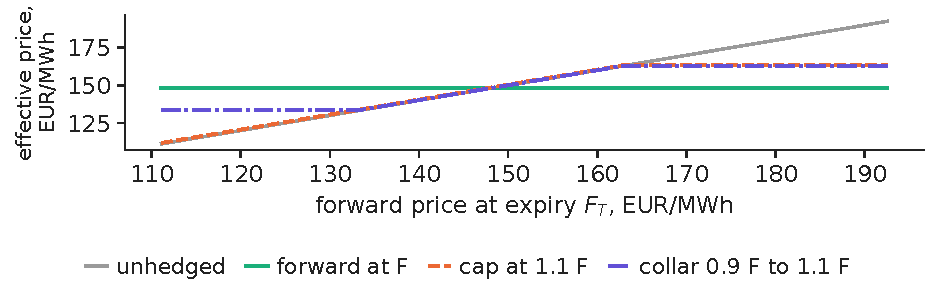
\includegraphics[width=\textwidth,height=0.477\textheight,keepaspectratio]{charts/en/collar.pdf}\end{center}\vspace{-3mm}
\chartsource{Source: OPCOM PCCB-LE-flex; ECB (€STR); Black-76. Data: F = Cal-2027 baseload, auctions 2026-09-01 to 2026-10-31.}
\vspace{0.5mm}
\begin{itemize}\setlength{\itemsep}{0pt}
  \item Forward 148.1
    \begin{itemize}\setlength{\itemsep}{0pt}
      \item Cap at 162.9 costs 0.63
      \item Collar 133.3 -- 162.9 costs 0.20 EUR/MWh
      \item Spikes and monthly averages (Asian options) break Black-76.
    \end{itemize}
\end{itemize}
\par\vfill\manager{a near-zero-cost collar lets a supplier sell a capped retail price.}\par\vspace{0.5mm}
\par\vfill\noindent{\scriptsize\color{FooterGray}(Black, 1976; Weron, 2008)}\hfill\qlink{EMQA\_L5\_collar}{Quantlets/L5/EMQA_L5_collar}\par\vspace{0.5mm}
\end{frame}


\section{Case study: a Romanian supplier and a producer}

\begin{frame}{Case study: a supplier with a 1 MW fixed-price customer in 2026}
\footnotesize
\begin{itemize}\setlength{\itemsep}{1pt}
  \item \textbf{The position}
    \begin{itemize}\setlength{\itemsep}{0pt}
      \item 1 MW flat for all of 2026 sold at a fixed price; energy still to be bought
      \item Measured on 10 delivered months, to Oct 2026
    \end{itemize}
  \item \textbf{Four strategies, real prices}
    \begin{itemize}\setlength{\itemsep}{0pt}
      \item Unhedged: buy each month at the realised spot mean
      \item 100\% forward: OPCOM band 2026, VWAP 111.70 EUR/MWh, 31 auctions
      \item 50\% forward, 50\% spot
      \item Monthly caps bought 15 Dec 2025, $K$ = 120.16 (VWAP of the last 5 auctions), Black-76, $\sigma$ = 0.668
    \end{itemize}
  \item \textbf{What we report}
    \begin{itemize}\setlength{\itemsep}{0pt}
      \item Mean cost, its month-to-month standard deviation, the worst month, total cost per MW
    \end{itemize}
\end{itemize}
\par\vfill\manager{a supplier's risk committee should see exactly this table every month.}\par\vspace{0.5mm}
\par\vfill\noindent{\scriptsize\color{FooterGray}(own computation; OPCOM)}\hfill\tryit{notebook \S7}\par\vspace{0.5mm}
\end{frame}

\begin{frame}{Case study: in 2026 the forward beat the spot in 6 of 10 months}
\small
\begin{center}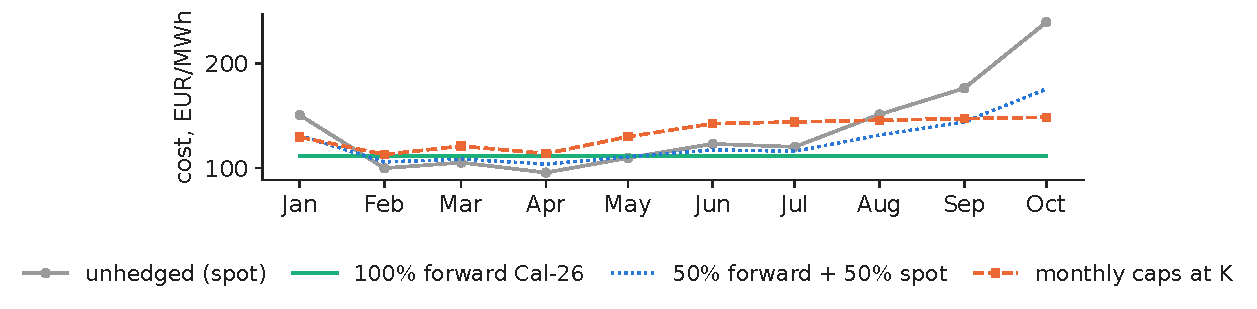
\includegraphics[width=\textwidth,height=0.564\textheight,keepaspectratio]{charts/en/case2026.pdf}\end{center}\vspace{-3mm}
\chartsource{Source: OPCOM (PCCB-LE-flex results; day-ahead prices via energy-charts.info); ECB. Data: 2026-01 to 2026-10; 1 MW baseload.}
\vspace{0.5mm}
\begin{itemize}\setlength{\itemsep}{0pt}
  \item Spot peak 239.3 EUR/MWh in Oct 2026
    \begin{itemize}\setlength{\itemsep}{0pt}
      \item The caps paid out in 5 of 10 months.
    \end{itemize}
\end{itemize}
\par\vfill\manager{a cap costs its premium every month, also when it pays nothing.}\par\vspace{0.5mm}
\par\vfill\noindent{\scriptsize\color{FooterGray}(own computation; OPCOM)}\hfill\qlink{EMQA\_L5\_case2026}{Quantlets/L5/EMQA_L5_case2026}\par\vspace{0.5mm}
\end{frame}

\begin{frame}{Case study: the forward cut cost and risk; the cap cut risk}
\footnotesize
\begin{columns}[T,onlytextwidth]
\begin{column}{0.50\textwidth}
{\footnotesize\renewcommand{\arraystretch}{1.25}\setlength{\tabcolsep}{4pt}
\begin{tabular}{@{}lrrrr@{}}\toprule
EUR/MWh & mean & st.\ dev. & worst & EUR/MW \\ \midrule
spot & 137.5 & 44.4 & 239.3 & 1\,002\,956 \\
100\% forward & 111.7 & 0.0 & 111.7 & 814\,946 \\
50\% forward & 124.6 & 22.2 & 175.5 & 908\,951 \\
caps & 133.6 & 13.9 & 148.5 & 975\,020 \\
\bottomrule\end{tabular}}
\par\vspace{0.5mm}{\scriptsize \begin{itemize}\setlength{\itemsep}{0pt}
  \item Weighted by the hours of each month.
\end{itemize}}
\end{column}
\begin{column}{0.47\textwidth}
\begin{itemize}\setlength{\itemsep}{1pt}
  \item \textbf{Reading}
    \begin{itemize}\setlength{\itemsep}{0pt}
      \item Forward: 188\,010 EUR per MW saved, zero variation
      \item Caps: premium 20.4 EUR/MWh a month; net 27\,936 EUR per MW
    \end{itemize}
  \item \textbf{Not a general verdict}
    \begin{itemize}\setlength{\itemsep}{0pt}
      \item Prices rose after the hedge; in a falling year the forward costs more than spot
    \end{itemize}
\end{itemize}
\end{column}
\end{columns}
\par\vfill\manager{set the hedged share by policy (e.g.\ 60--80\% bought in layers), not by a price view.}\par\vspace{0.5mm}
\par\vfill\noindent{\scriptsize\color{FooterGray}(own computation)}\hfill\tryit{notebook \S7}\par\vspace{0.5mm}
\end{frame}

\begin{frame}{The producer's side, and the summer 2024 spike}
\footnotesize
\begin{itemize}\setlength{\itemsep}{1pt}
  \item \textbf{Producer, 2025}
    \begin{itemize}\setlength{\itemsep}{0pt}
      \item 101 auctions, VWAP 102.1 vs realised 108.2 EUR/MWh
      \item Selling forward earned 6.0 EUR/MWh less than spot (52\,797 EUR per MW-year), the price of a fixed revenue
      \item In 2022 the same decision cost 187.9 EUR/MWh
    \end{itemize}
  \item \textbf{Summer 2024}
    \begin{itemize}\setlength{\itemsep}{0pt}
      \item Third quarter bought at 90.0, delivered at 127.4 EUR/MWh; July alone 145.1
      \item Peak hour 916.7 EUR/MWh on 18 Jul 2024, 20:00, Central European Time (CET)
    \end{itemize}
  \item \textbf{The lesson}
    \begin{itemize}\setlength{\itemsep}{0pt}
      \item A hedge transfers value between the two sides; it makes cash flows predictable, which lenders pay for
    \end{itemize}
\end{itemize}
\par\vfill\manager{a producer with debt should sell forward even when it expects higher prices.}\par\vspace{0.5mm}
\par\vfill\noindent{\scriptsize\color{FooterGray}(own computation; OPCOM; Andrei, Pele \& Cramer, 2026, PICBE)}\hfill\tryit{notebook \S7}\par\vspace{0.5mm}
\end{frame}

\begin{frame}{Elements of a hedging policy}
\footnotesize
\begin{columns}[T,onlytextwidth]
\begin{column}{0.50\textwidth}
\begin{itemize}\setlength{\itemsep}{1pt}
  \item \textbf{Exposure}
    \begin{itemize}\setlength{\itemsep}{0pt}
      \item Net position per month and profile (band, peak, solar)
      \item Volume risk: demand hardly reacts to price
    \end{itemize}
  \item \textbf{Instruments}
    \begin{itemize}\setlength{\itemsep}{0pt}
      \item OPCOM forwards first, then Hungarian, then German futures
      \item Caps for the tail, not for all the volume
    \end{itemize}
\end{itemize}
\end{column}
\begin{column}{0.47\textwidth}
\begin{itemize}\setlength{\itemsep}{1pt}
  \item \textbf{Execution}
    \begin{itemize}\setlength{\itemsep}{0pt}
      \item Buy in layers over 12--24 months
      \item Keep a liquidity buffer for margin calls
    \end{itemize}
  \item \textbf{Control}
    \begin{itemize}\setlength{\itemsep}{0pt}
      \item Limits on open position and VaR (Lecture 4)
      \item Report hedged cost and its variance
    \end{itemize}
\end{itemize}
\end{column}
\end{columns}
\par\vfill\manager{the board approves the policy, traders execute it, risk management measures it.}\par\vspace{0.5mm}
\par\vfill\noindent{\scriptsize\color{FooterGray}(Hull, 2022; Proșcanu, Proșcanu \& Pele, 2025, JSES; Lecture 4)}\par\vspace{0.5mm}
\end{frame}

\section*{Wrap-up}

\begin{frame}{Quiz 1: basis risk}
\small
\begin{itemize}
  \item A Romanian supplier hedged July 2024 with German baseload futures bought at $F$
    \begin{itemize}\setlength{\itemsep}{0pt}
      \item July averaged 67.7 in Germany and 145.1 EUR/MWh in Romania
      \item What did it pay per MWh?
    \end{itemize}
\end{itemize}
\vspace{2mm}
\begin{exampleblock}{Answer}
\begin{itemize}
  \item It bought at 145.1 in Romania and received from the future the difference between 67.7 and $F$: net cost $F$ + 77.4 EUR/MWh, the largest monthly basis in our data.
\end{itemize}
\end{exampleblock}
\end{frame}

\begin{frame}{Quiz 2: the hedge ratio}
\small
\begin{itemize}
  \item Our estimate for Hungary is $h^{*}$ = 0.966 with a bootstrap interval [0.93; 1.03]
    \begin{itemize}\setlength{\itemsep}{0pt}
      \item A 20 MW exposure needs how many MW of Hungarian futures?
    \end{itemize}
\end{itemize}
\vspace{2mm}
\begin{exampleblock}{Answer}
\begin{itemize}
  \item 20 $\times$ 0.966 = 19.3 MW
    \begin{itemize}\setlength{\itemsep}{0pt}
      \item Since 1 lies inside the interval, a one-for-one hedge of 20 MW is statistically as good.
    \end{itemize}
\end{itemize}
\end{exampleblock}
\end{frame}

\begin{frame}{Quiz 3: spark spread}
\small
\begin{itemize}
  \item In Oct 2026: power 239.3, gas 86.8 EUR/MWh, EUA 82.4 EUR/t
    \begin{itemize}\setlength{\itemsep}{0pt}
      \item Efficiency 50\%, 0.202 t CO$_2$ per MWh thermal
      \item Did a gas plant earn money on average?
    \end{itemize}
\end{itemize}
\vspace{2mm}
\begin{exampleblock}{Answer}
\begin{itemize}
  \item Fuel 86.8/0.5 = 173.6
    \begin{itemize}\setlength{\itemsep}{0pt}
      \item Carbon 0.404 $\times$ 82.4 = 33.3
      \item Clean spark \ensuremath{+}32.4 EUR/MWh: yes, even before choosing the best hours.
    \end{itemize}
\end{itemize}
\end{exampleblock}
\end{frame}

\begin{frame}{Quiz 4: a cap for a supplier}
\small
\begin{itemize}
  \item The 2027 band trades at 148.1
    \begin{itemize}\setlength{\itemsep}{0pt}
      \item A cap at 162.9 costs 0.63 EUR/MWh
      \item What does the supplier pay if the forward ends at 1.3 $F$, and at 0.9 $F$?
    \end{itemize}
\end{itemize}
\vspace{2mm}
\begin{exampleblock}{Answer}
\begin{itemize}
  \item At 1.3 $F$: the strike 162.9 plus the premium
    \begin{itemize}\setlength{\itemsep}{0pt}
      \item At 0.9 $F$: the market price plus the premium, since the cap is not exercised.
    \end{itemize}
\end{itemize}
\end{exampleblock}
\end{frame}

\begin{frame}{Wrap-up}
\small
\vspace{-2mm}\begin{multicols}{2}\scriptsize\tableofcontents\end{multicols}
\begin{itemize}\setlength{\itemsep}{1pt}
  \item A forward turns an unknown spot into a known price
    \begin{itemize}\setlength{\itemsep}{0pt}
      \item In 2022 it saved a Romanian supplier 1.65 million EUR per MW, and cost producers the same.
    \end{itemize}
  \item Hedge Romania with Hungary before Germany, price the shape, and match the volatility to the underlying
    \begin{itemize}\setlength{\itemsep}{0pt}
      \item Next: Lecture 6.
    \end{itemize}
\end{itemize}
\end{frame}

\begin{frame}{Research from our group on Romanian power risk}
\footnotesize
\begin{itemize}\setlength{\itemsep}{1pt}
  \item \textbf{The summer 2024 price spike} (Andrei, Pele \& Cramer, 2026, PICBE)
    \begin{itemize}\setlength{\itemsep}{0pt}
      \item Question: which intervention would have lowered Romanian prices most in June--July 2024
      \item Method: a random forest on hourly ENTSO-E data, 147 counterfactual scenarios, checked against ridge regression
      \item Result: a 10\% load reduction was the most effective measure; the peak came at night, so solar could not help and storage is the enabling asset
    \end{itemize}
  \item \textbf{Systemic risk in the EU energy sector} (Toma, Dima, Grecu, Pele \& Lessmann, 2026, SSRN)
    \begin{itemize}\setlength{\itemsep}{0pt}
      \item Method: the Energy Financial Risk Meter, a least absolute shrinkage and selection operator (LASSO) quantile regression on daily returns of 100 European energy companies
      \item Result: the index captures the 2020 pandemic and the 2022 war; a geopolitical-to-energy risk channel switched on
    \end{itemize}
  \item \textbf{Demand barely reacts to price} (Proșcanu, Proșcanu \& Pele, 2025, JSES)
    \begin{itemize}\setlength{\itemsep}{0pt}
      \item Method: Granger causality and vector autoregressions on Romanian consumption and prices
      \item Result: consumption is inelastic and drives price, not the reverse, so volume cannot hedge price risk
    \end{itemize}
\end{itemize}
\par\vspace{0.5mm}{\scriptsize \begin{itemize}\setlength{\itemsep}{0pt}
  \item Findings as stated in the papers; numbers on the other slides come from our own data.
\end{itemize}}
\par\vfill\noindent{\scriptsize\color{FooterGray}(Bucharest University of Economic Studies; Romanian Academy, Institute for Economic Forecasting)}\par\vspace{0.5mm}
\end{frame}

\begin{frame}{Want to learn more?}
\small
\begin{columns}[T,onlytextwidth]
\begin{column}{0.52\textwidth}
\begin{itemize}\setlength{\itemsep}{1pt}
  \item \textbf{J.\ Hull, Options, Futures, and Other Derivatives}, chapters on hedging, futures and Black's model.
  \item \textbf{Benth, Šaltytė Benth \& Koekebakker (2008)}: forward curves and options in electricity markets.
  \item \textbf{OPCOM reports}: forward auction results, the source of this lecture --- \href{https://www.opcom.ro/rapoarte-pccb-le-flex-rez-pccb-le-flex/ro}{opcom.ro}.
\end{itemize}
\end{column}
\begin{column}{0.45\textwidth}
\begin{itemize}\setlength{\itemsep}{1pt}
  \item \textbf{This course}: code, data, notebooks --- \href{https://github.com/danpele/EMQA}{github.com/danpele/EMQA}.
  \item \textbf{ACER (2022)}: the final assessment of the EU wholesale electricity market design.
  \item \textbf{Experiment yourself}: the notebook reproduces every chart and number of this lecture --- \href{\emqarepo/\emqanb}{notebooks/}.
\end{itemize}
\end{column}
\end{columns}
\end{frame}

\begin{frame}{References (1/3)}
\scriptsize
\begin{itemize}\setlength{\itemsep}{1pt}\scriptsize
\item ACER (2022). \textit{ACER's Final Assessment of the EU Wholesale Electricity Market Design}. Ljubljana, April 2022. \href{https://www.acer.europa.eu/events-and-engagement/news/press-release-acer-publishes-its-final-assessment-eu-wholesale}{acer.europa.eu}
\item Andrei, A.-V., Pele, D.-T.\ \& Cramer, A.-A.\ (2026). Evaluating intervention effectiveness during extreme price events: A counterfactual analysis of Romania's 2024 energy crisis. \textit{Proceedings of the International Conference on Business Excellence}, 20(1), 84--103. \href{https://doi.org/10.2478/picbe-2026-0013}{doi:10.2478/picbe-2026-0013}
\item Benth, F.\,E., Šaltytė Benth, J.\ \& Koekebakker, S.\ (2008). \textit{Stochastic Modeling of Electricity and Related Markets}. World Scientific. \href{https://doi.org/10.1142/6811}{doi:10.1142/6811}
\item Bessembinder, H.\ \& Lemmon, M.\,L.\ (2002). Equilibrium pricing and optimal hedging in electricity forward markets. \textit{Journal of Finance}, 57(3), 1347--1382. \href{https://doi.org/10.1111/1540-6261.00463}{doi:10.1111/1540-6261.00463}
\item Black, F.\ (1976). The pricing of commodity contracts. \textit{Journal of Financial Economics}, 3(1--2), 167--179. \href{https://doi.org/10.1016/0304-405X(76)90024-6}{doi:10.1016/0304-405X(76)90024-6}
\item Deng, S.-J., Johnson, B.\ \& Sogomonian, A.\ (2001). Exotic electricity options and the valuation of electricity generation and transmission assets. \textit{Decision Support Systems}, 30(3), 383--392. \href{https://doi.org/10.1016/S0167-9236(00)00112-3}{doi:10.1016/S0167-9236(00)00112-3}
\item Ederington, L.\,H.\ (1979). The hedging performance of the new futures markets. \textit{Journal of Finance}, 34(1), 157--170. \href{https://doi.org/10.1111/j.1540-6261.1979.tb02077.x}{doi:10.1111/j.1540-6261.1979.tb02077.x}
\item ENTSO-E (2021). Successful go-live of Interim Coupling, reaching the SDAC enduring phase. Press release, 18 June 2021. \href{https://www.entsoe.eu/news/2021/06/18/successful-go-live-of-interim-coupling-reaching-the-sdac-enduring-phase/}{entsoe.eu}
\end{itemize}
\end{frame}

\begin{frame}{References (2/3)}
\scriptsize
\begin{itemize}\setlength{\itemsep}{1pt}\scriptsize
\item Eydeland, A.\ \& Wolyniec, K.\ (2003). \textit{Energy and Power Risk Management: New Developments in Modeling, Pricing, and Hedging}. Wiley. \href{https://www.wiley.com/en-us/Energy+and+Power+Risk+Management-p-9780471104001}{wiley.com}
\item Fama, E.\,F.\ \& French, K.\,R.\ (1987). Commodity futures prices: Some evidence on forecast power, premiums, and the theory of storage. \textit{Journal of Business}, 60(1), 55--73. \href{https://doi.org/10.1086/296385}{doi:10.1086/296385}
\item Hull, J.\,C.\ (2022). \textit{Options, Futures, and Other Derivatives}, 11th ed. Pearson. \href{https://www.pearson.com/en-us/subject-catalog/p/options-futures-and-other-derivatives/P200000005938}{pearson.com}
\item IPCC (2006). \textit{2006 IPCC Guidelines for National Greenhouse Gas Inventories}, Vol.\ 2 Energy, ch.\ 2, Table 2.2 (default emission factors). \href{https://www.ipcc-nggip.iges.or.jp/public/2006gl/pdf/2_Volume2/V2_2_Ch2_Stationary_Combustion.pdf}{ipcc-nggip.iges.or.jp}
\item Johnson, L.\,L.\ (1960). The theory of hedging and speculation in commodity futures. \textit{Review of Economic Studies}, 27(3), 139--151. \href{https://doi.org/10.2307/2296076}{doi:10.2307/2296076}
\item Kroner, K.\,F.\ \& Sultan, J.\ (1993). Time-varying distributions and dynamic hedging with foreign currency futures. \textit{Journal of Financial and Quantitative Analysis}, 28(4), 535--551. \href{https://doi.org/10.2307/2331164}{doi:10.2307/2331164}
\item Longstaff, F.\,A.\ \& Wang, A.\,W.\ (2004). Electricity forward prices: A high-frequency empirical analysis. \textit{Journal of Finance}, 59(4), 1877--1900. \href{https://doi.org/10.1111/j.1540-6261.2004.00682.x}{doi:10.1111/j.1540-6261.2004.00682.x}
\item Margrabe, W.\ (1978). The value of an option to exchange one asset for another. \textit{Journal of Finance}, 33(1), 177--186. \href{https://doi.org/10.1111/j.1540-6261.1978.tb03397.x}{doi:10.1111/j.1540-6261.1978.tb03397.x}
\end{itemize}
\end{frame}

\begin{frame}{References (3/3)}
\scriptsize
\begin{itemize}\setlength{\itemsep}{1pt}\scriptsize
\item OUG 27/2022 privind măsurile aplicabile clienților finali din piața de energie electrică și gaze naturale (Monitorul Oficial nr.\ 274, 22 martie 2022); OUG 153/2022 (MACEE). \href{https://legislatie.just.ro}{legislatie.just.ro}
\item Proșcanu, C., Proșcanu, M.\ \& Pele, D.\,T.\ (2025). The price elasticity of electricity demand in Romania. \textit{Journal of Social and Economic Statistics}, 14(2), 131--141. \href{https://doi.org/10.2478/jses-2025-0009}{doi:10.2478/jses-2025-0009}
\item Redl, C., Haas, R., Huber, C.\ \& Böhm, B.\ (2009). Price formation in electricity forward markets and the relevance of systematic forecast errors. \textit{Energy Economics}, 31(3), 356--364. \href{https://doi.org/10.1016/j.eneco.2008.12.001}{doi:10.1016/j.eneco.2008.12.001}
\item Samuelson, P.\,A.\ (1965). Proof that properly anticipated prices fluctuate randomly. \textit{Industrial Management Review}, 6(2), 41--49; reprinted in \textit{World Scientific Handbook in Financial Economics} (2015), 25--38. \href{https://doi.org/10.1142/9789814566926_0002}{doi:10.1142/9789814566926\_0002}
\item Schwartz, E.\,S.\ (1997). The stochastic behavior of commodity prices: Implications for valuation and hedging. \textit{Journal of Finance}, 52(3), 923--973. \href{https://doi.org/10.1111/j.1540-6261.1997.tb02721.x}{doi:10.1111/j.1540-6261.1997.tb02721.x}
\item Toma, F.-M., Dima, D.\,M., Grecu, R., Pele, D.\,T.\ \& Lessmann, S.\ (2026). Energy Financial Risk Meter: Systemic risk in the EU energy sector. SSRN working paper. \href{https://doi.org/10.2139/ssrn.6985301}{doi:10.2139/ssrn.6985301}
\item Weron, R.\ (2008). Market price of risk implied by Asian-style electricity options and futures. \textit{Energy Economics}, 30(3), 1098--1115. \href{https://doi.org/10.1016/j.eneco.2007.05.004}{doi:10.1016/j.eneco.2007.05.004}
\end{itemize}
\end{frame}

\appendix

\section*{Appendix}

\begin{frame}{Appendix A: the minimum-variance hedge ratio and its estimation}
\small
\begin{columns}[T,onlytextwidth]
\begin{column}{0.54\textwidth}
\[ \frac{\partial}{\partial h}\Var(\Delta S-h\Delta F)=-2\Cov(\Delta S,\Delta F)+2h\Var(\Delta F)=0 \]\[ \Rightarrow\ h^{*}=\frac{\Cov(\Delta S,\Delta F)}{\Var(\Delta F)} \]\[ \Var(\Delta S-h^{*}\Delta F)=\sigma_S^2(1-\rho^2) \]\begin{itemize}\setlength{\itemsep}{1pt}
  \item The second derivative $2\Var(\Delta F)>0$, so $h^{*}$ is a minimum.
  \item $h^{*}$ is the OLS slope of $\Delta S$ on $\Delta F$
    \begin{itemize}\setlength{\itemsep}{0pt}
      \item HAC variance (Newey--West, Bartlett kernel, 3 lags).
    \end{itemize}
\end{itemize}
\end{column}
\begin{column}{0.43\textwidth}
\begin{itemize}\setlength{\itemsep}{1pt}
  \item \textbf{Moving-block bootstrap}
    \begin{itemize}\setlength{\itemsep}{0pt}
      \item Draw blocks of 6 consecutive months with replacement until $n$ months; recompute $h^{*}$; repeat 2\,000 times
      \item 95\% interval = 2.5\% and 97.5\% percentiles; blocks keep the autocorrelation of the monthly changes
    \end{itemize}
  \item \textbf{Dynamic hedge ratios}
    \begin{itemize}\setlength{\itemsep}{0pt}
      \item $h_t^{*}=\Cov_{t-1}/\Var_{t-1}$ from a bivariate GARCH (Lecture 3)
    \end{itemize}
\end{itemize}
\end{column}
\end{columns}
\par\vfill\noindent{\scriptsize\color{FooterGray}(Johnson, 1960; Ederington, 1979; Kroner \& Sultan, 1993)}\par\vspace{0.5mm}
\end{frame}

\begin{frame}{Appendix B: from a driftless forward to the Black-76 formula}
\small
\begin{columns}[T,onlytextwidth]
\begin{column}{0.54\textwidth}
\[ \frac{dF_t}{F_t}=\sigma\,dW_t\ \Rightarrow\ \ln F_T\sim\mathcal N\big(\ln F_0-\tfrac12\sigma^2T,\ \sigma^2T\big) \]\[ C=e^{-rT}\E\big[(F_T-K)^+\big]=e^{-rT}\big[F_0\Phi(d_1)-K\Phi(d_2)\big] \]\begin{itemize}\setlength{\itemsep}{1pt}
  \item A forward costs nothing to enter, so under the pricing measure its drift is zero.
  \item $\E[F_T\mathbf 1_{F_T>K}]=F_0\Phi(d_1)$ and $\Pr(F_T>K)=\Phi(d_2)$ (lognormal moments).
\end{itemize}
\end{column}
\begin{column}{0.43\textwidth}
\begin{itemize}\setlength{\itemsep}{1pt}
  \item \textbf{Spread options}
    \begin{itemize}\setlength{\itemsep}{0pt}
      \item An option to exchange gas for power: Margrabe's formula with $\sigma^2=\sigma_P^2+\sigma_G^2-2\rho\sigma_P\sigma_G$
      \item With a strike (clean spark with fixed costs) Kirk's approximation is used in practice
    \end{itemize}
  \item \textbf{Mean reversion}
    \begin{itemize}\setlength{\itemsep}{0pt}
      \item Spot power reverts to its mean; Schwartz (1997) one-factor model gives forward volatilities that fall with maturity
    \end{itemize}
\end{itemize}
\end{column}
\end{columns}
\par\vfill\noindent{\scriptsize\color{FooterGray}(Black, 1976; Margrabe, 1978; Schwartz, 1997)}\par\vspace{0.5mm}
\end{frame}

\begin{frame}{Appendix C: conventions and conversion factors}
\footnotesize
\begin{itemize}\setlength{\itemsep}{1pt}
  \item \textbf{Forward prices}
    \begin{itemize}\setlength{\itemsep}{0pt}
      \item One closing price per OPCOM session; quantity on the initiator side; lei converted with the ECB EUR/RON fixing of the auction day (last fixing on or before)
      \item Standard periods only: month, quarter, half-year, calendar year; baseload unless stated
    \end{itemize}
  \item \textbf{Realised spot}
    \begin{itemize}\setlength{\itemsep}{0pt}
      \item Mean of the daily day-ahead base prices of the delivery period (CET days); computed only when every day is present
    \end{itemize}
  \item \textbf{Fuels and carbon}
    \begin{itemize}\setlength{\itemsep}{0pt}
      \item Coal 6\,000 kcal/kg = 6.978 MWh thermal per tonne; gas 0.202 and hard coal 0.341 t CO$_2$ per MWh thermal (IPCC 2006: 56.1 and 94.6 t/TJ)
      \item EUA = EEX auction monthly mean to Jan 2026, then SparkChange ETC (auction/ETC ratio close to 1 in 2021--2025)
    \end{itemize}
  \item \textbf{Hours}
    \begin{itemize}\setlength{\itemsep}{0pt}
      \item Hour-equivalents: a 15-minute interval counts 0.25 h (since 1 October 2025)
    \end{itemize}
\end{itemize}
\par\vfill\noindent{\scriptsize\color{FooterGray}(IPCC, 2006; OPCOM; ECB)}\par\vspace{0.5mm}
\end{frame}

\end{document}
